\documentclass[11pt,oneside]{book}

\usepackage[T1]{fontenc}
\usepackage[utf8]{inputenc}
\usepackage{lmodern}
\usepackage[margin=0.90in]{geometry}
\usepackage{amsmath,amssymb,mathtools}
\usepackage{proof}
\usepackage{listings}
\usepackage{xcolor}
\usepackage{booktabs,longtable,array}
\usepackage{enumitem}
\usepackage{microtype}
\usepackage{tikz}
\usetikzlibrary{arrows.meta,positioning,fit,shapes.geometric}
\usepackage{hyperref}

\hypersetup{
  colorlinks=true,
  linkcolor=blue!45!black,
  citecolor=green!35!black,
  urlcolor=magenta!45!black,
  pdftitle={From Separation Logic to a Checked Cyclic Certificate},
  pdfauthor={Cyclist Rocq project documentation}
}
\setcounter{tocdepth}{2}
\setcounter{secnumdepth}{3}
\setlength{\emergencystretch}{2em}
\renewcommand{\arraystretch}{1.12}
\linespread{1.04}

\definecolor{rocqblue}{RGB}{25,74,135}
\definecolor{rocqgreen}{RGB}{34,120,82}
\definecolor{rocqgray}{RGB}{95,99,104}
\definecolor{rocqback}{RGB}{247,248,250}
\lstdefinelanguage{Rocq}{
  morekeywords={From,Require,Import,Definition,Fixpoint,Inductive,Record,
    Module,Type,Parameter,End,Lemma,Theorem,Example,Proof,Qed,Defined,
    match,with,end,fun,forall,exists,let,in,if,then,else,return,as,
    destruct,intros,apply,exact,refine,unfold,rewrite,simpl,pose,set},
  sensitive=true,
  morecomment=[s]{(*}{*)},
  morestring=[b]"
}
\lstdefinestyle{rocq}{
  language=Rocq,
  basicstyle=\ttfamily\small,
  keywordstyle=\color{rocqblue}\bfseries,
  commentstyle=\color{rocqgreen},
  stringstyle=\color{magenta!60!black},
  numbers=left,
  numberstyle=\scriptsize\color{rocqgray},
  numbersep=8pt,
  frame=single,
  rulecolor=\color{black!18},
  backgroundcolor=\color{rocqback},
  breaklines=true,
  breakatwhitespace=false,
  columns=fullflexible,
  keepspaces=true,
  showstringspaces=false,
  tabsize=2,
  captionpos=b
}
\lstset{style=rocq}

\DeclareRobustCommand{\code}[1]{\texttt{\detokenize{#1}}}
\DeclareRobustCommand{\file}[1]{\texttt{\detokenize{#1}}}
\newcommand{\src}[2]{\code{#2} in \file{#1}}
\newcommand{\Nat}{\mathbb{N}}
\newcommand{\sem}[1]{[\![#1]\!]}
\newcommand{\holds}{\models}
\newcommand{\notholds}{\not\models}
\newcommand{\uplusd}{\mathbin{\uplus}}
\newcommand{\pto}{\mathbin{\mapsto}}
\newcommand{\slstar}{\mathbin{*}}
\newcommand{\Valid}{\mathsf{Valid}}
\newcommand{\rank}{\mathsf{rank}}
\newcommand{\mathintent}{\subsection*{Mathematical intention}}
\newcommand{\rocqreal}{\subsection*{Rocq realization}}
\newcommand{\soundlim}{\subsection*{Soundness and limitations}}
\newcommand{\takeaway}[1]{\begin{quote}\small\textbf{Reading invariant.} #1\end{quote}}

\title{\textbf{From Separation Logic to a Checked Cyclic Certificate}\\[0.7em]
  A Theory-to-Code Tutorial for \file{Rocq-copy/SP}}
\author{Cyclist Rocq project documentation}
\date{Source revision\\\code{08f6cd8834a3fc22088a064025abb9ee65c7f545}}

\begin{document}
\hypersetup{pageanchor=false}
\frontmatter
\maketitle
\hypersetup{pageanchor=true}

\chapter*{Purpose and reader contract}
\addcontentsline{toc}{chapter}{Purpose and reader contract}

This tutorial is for a separation-logic researcher who already reads Rocq but
wants to understand exactly what theorem the \file{SP} implementation proves,
how executable search reaches that theorem, and where the current prover stops.
The exposition proceeds from mathematics to representation to trusted theorem.
It does not teach Gallina syntax, and it does not infer features from
\file{SP/IMPLEMENTATION_PLAN.md} that are absent from the checked source.

The implementation is small enough to audit---twelve \file{SP} modules and two
generic \file{Cyclic} modules---but it crosses several conceptual boundaries:
finite-heap semantics, finite approximants of inductive predicates, local rule
soundness, finite cyclic graphs, global trace progress, reflection, and bounded
depth-first search.  The main discipline of this document is therefore:

\begin{center}
\fbox{\parbox{0.87\textwidth}{Every executable success is followed to a
kernel-checked semantic theorem; every executable failure is described only as
bounded non-success.}}
\end{center}

Selected excerpts reproduce the revision named on the title page.  A source
reference such as \src{SP/Semantics.v}{predicate_holds_rank} names both the
module and the symbol to inspect.  The source remains authoritative.

\tableofcontents

\mainmatter

\chapter{Orientation: the theorem-producing path}
\label{ch:orientation}

\mathintent

An automated entailment prover should not merely return ``yes.''  Its useful
output is a derivation object whose acceptance implies semantic validity.  For
this project, the complete path is
\[
 \boxed{\text{judgment}}
 \longrightarrow \boxed{\text{generator}}
 \longrightarrow \boxed{\text{proof graph}}
 \longrightarrow \boxed{\text{checks}}
 \longrightarrow \boxed{\text{certificate}}
 \longrightarrow \boxed{\text{semantic validity}}.
\]
Each arrow changes the kind of evidence.  A judgment is reified syntax.  A
generator may return only theorem-backed rule packages.  Search connects those
packages into a finite graph.  Boolean checks validate finite structure and
progress data.  Reflection turns a successful equation into dependent semantic
evidence.  Finally, a generic well-founded argument rules out a countermodel at
the root.

This architecture follows the separation between an object logic and a generic
cyclic engine explored in cyclic proof theory and in Cyclist
\cite{brotherston2011sequent,brotherston2012generic}.  The object logic must say
what a world is, what a judgment means, and what measure a trace follows.  The
generic layer need not know what a heap or an inductive predicate is.

\rocqreal

Figure~\ref{fig:dependency-map} is the module map.  Solid arrows mean a direct
logical dependency in the relevant build path.  Dashed arrows show clients used
for examples or regression tests.  Every \file{SP/*.v} module appears.

\begin{figure}[p]
\centering
\resizebox{\textwidth}{!}{%
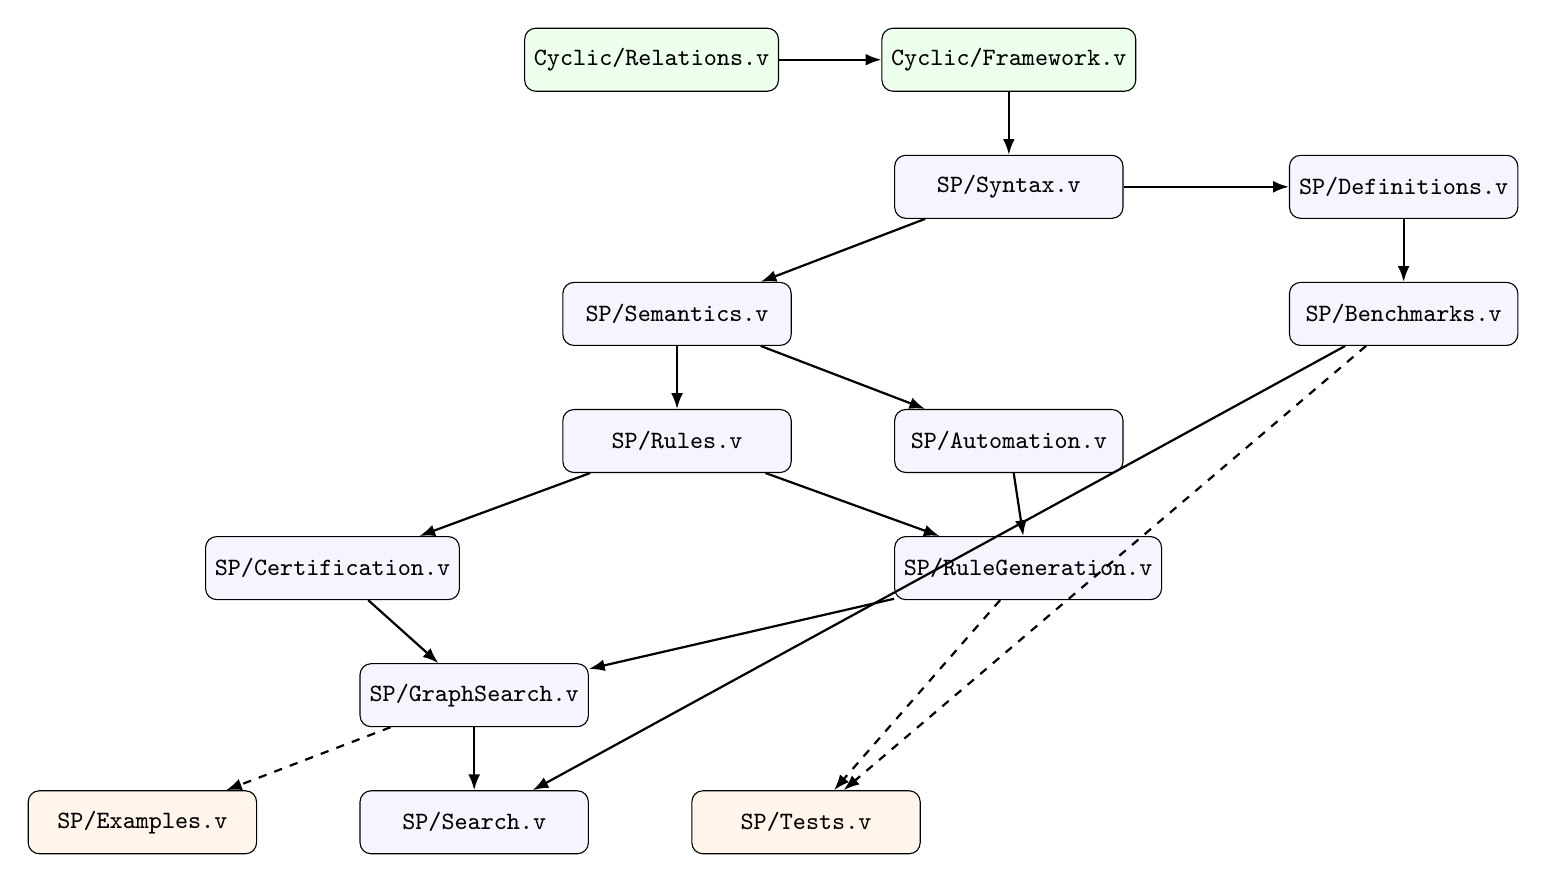
\begin{tikzpicture}[
  node distance=8mm and 13mm,
  box/.style={draw,rounded corners,align=center,minimum width=29mm,
              minimum height=8mm,fill=blue!4,font=\small\ttfamily},
  cbox/.style={box,fill=green!7},
  client/.style={box,fill=orange!8},
  arr/.style={-{Latex[length=2mm]},thick},
  darr/.style={arr,dashed}
]
\node[cbox] (rel) {Cyclic/Relations.v};
\node[cbox,right=of rel] (fw) {Cyclic/Framework.v};
\node[box,below=of fw] (syn) {SP/Syntax.v};
\node[box,below left=of syn] (sem) {SP/Semantics.v};
\node[box,below=of sem] (rules) {SP/Rules.v};
\node[box,right=of rules] (auto) {SP/Automation.v};
\node[box,below left=of rules] (cert) {SP/Certification.v};
\node[box,below right=of rules] (gen) {SP/RuleGeneration.v};
\node[box,below=of cert,xshift=18mm] (graph) {SP/GraphSearch.v};
\node[box,right=of syn,xshift=8mm] (defs) {SP/Definitions.v};
\node[box,below=of defs] (bench) {SP/Benchmarks.v};
\node[box,below=of graph] (search) {SP/Search.v};
\node[client,left=of search] (examples) {SP/Examples.v};
\node[client,right=of search] (tests) {SP/Tests.v};

\draw[arr] (rel) -- (fw);
\draw[arr] (fw) -- (syn);
\draw[arr] (syn) -- (sem);
\draw[arr] (sem) -- (rules);
\draw[arr] (sem) -- (auto);
\draw[arr] (rules) -- (cert);
\draw[arr] (rules) -- (gen);
\draw[arr] (auto) -- (gen);
\draw[arr] (cert) -- (graph);
\draw[arr] (gen) -- (graph);
\draw[arr] (syn) -- (defs);
\draw[arr] (defs) -- (bench);
\draw[arr] (graph) -- (search);
\draw[arr] (bench) -- (search);
\draw[darr] (graph) -- (examples);
\draw[darr] (gen) -- (tests);
\draw[darr] (bench) -- (tests);
\end{tikzpicture}
}
\caption{Complete module map for the documented \file{SP} implementation and
the required generic \file{Cyclic} substrate.}
\label{fig:dependency-map}
\end{figure}

At the public boundary, \src{SP/Search.v}{search_sound} has the form
\[
  \mathsf{solvedb}(c,J)=\mathsf{true}\quad\Longrightarrow\quad \Valid(J).
\]
Here \(\Valid(J)\) is not another Boolean: it abbreviates
\(\forall w,\sem{J}(w)\).  Chapter~\ref{ch:search} traces the implementation of
this implication.

\soundlim

The direction is intentionally one-way.  Successful search provides a proof;
unsuccessful bounded search provides no countermodel and establishes no
negation.  Moreover, the path is proof-producing only because generators return
records containing proofs.  A graph node never receives an unproved rule name
that the checker later interprets on trust.

The \file{Cyclic} layer also runs two notions of global progress: a relational
closure check and a concrete finite trace-witness check.  Both are required for
acceptance, but only the witness is projected into the semantic certificate.
This deliberate distinction is developed in Chapters~\ref{ch:cyclic} and
\ref{ch:reflection}.

\chapter{Reified symbolic heaps}
\label{ch:syntax}

\mathintent

Fix a countable set of locations, with a distinguished null location.  Terms
are either null or variables.  Variables have two roles: free variables obtain
their value from the ambient world, while existential variables obtain their
value from a witness chosen when a formula is satisfied.

A symbolic heap has the conventional shape
\[
  \Pi \;\land\; \Sigma,
  \qquad
  \Sigma = A_1 \slstar \cdots \slstar A_n,
\]
where \(\Pi\) is a conjunction of equalities and disequalities, and each spatial
atom is either a points-to cell or an inductive predicate occurrence.  This
implementation stores points-to atoms and predicate atoms in separate lists.
A formula is
\[
  C\;\land\;(H_1\lor\cdots\lor H_k),
\]
where \(C\) is a conjunction of constraints between trace-tag bounds.  The
empty list of disjuncts denotes false; the one-element formula containing an
atom-free symbolic heap denotes \(emp\).

Tags are proof annotations on predicate occurrences, not part of predicate
membership.  A tag is anonymous, free, or existential.  Named tags may occur
in strict or non-strict ordinal constraints.  An inductive definition maps a
predicate name to clauses \(B(\bar{x},\bar{z}) \Rightarrow P(\bar{x})\), with
the extra variables \(\bar z\) local to a clause instance.

\rocqreal

The central records in \file{SP/Syntax.v} preserve these layers rather than
flattening them:

\begin{lstlisting}[caption={The reified symbolic-heap core.}]
Record symheap : Type := {
  heap_pure : list pure_atom;
  heap_points : list points_to;
  heap_predicates : list tagged_predicate
}.

Record formula : Type := {
  formula_constraints : list ordinal_constraint;
  formula_heaps : list symheap
}.

Record sequent : Type := {
  antecedent : formula;
  succedent : formula
}.
\end{lstlisting}

The excerpt realizes the mathematical shape above: list conjunction is used
inside a heap and list disjunction at formula level.  Definitions are reified
as \code{list (string * list clause)}, and a \code{judgment} packages the
definition environment together with its sequent.  Consequently equality of
judgments includes equality of the entire definition environment.

All syntax has decidable structural equality.  In particular,
\src{SP/Syntax.v}{judgment_eqb_spec} reflects a successful Boolean comparison
to propositional equality.  The graph builder relies on this exact equality
when installing an axiom or rule.  \src{SP/Syntax.v}{backlink_eqb} is different:
it first erases predicate tags and formula constraints but retains definitions,
terms, predicates, points-to atoms, and disjunct structure.  This relaxed test
does not itself justify a backlink; the backlink still carries a theorem-backed
unary rule.

Term substitutions are association lists.  \src{SP/Syntax.v}{unify_term} is a
one-way matcher: \code{Nil} matches only \code{Nil}, whereas any pattern
\code{Var x} may be bound to the target term.  A repeated variable must receive
the same target.  Tag substitutions are separate, so a term match can never
silently change trace annotations.  Freshening shifts only existential
identifiers; free parameters retain their identity.

The visible trace tags of a judgment are computed by
\src{SP/Syntax.v}{judgment_tags}.  Only \code{FreeTag n} occurrences in the
antecedent are exposed.  Anonymous and existential tags are not framework trace
identifiers.

\soundlim

The representation is deliberately intensional.  Spatial atoms are not sorted,
equalities are not solved, and disjuncts are not canonicalized.  At this
revision, all four normalization functions are the identity.  Thus two
mathematically equivalent heaps need not be structurally equal or match the
same generator.  This incompleteness is safe: structural equality is used to
restrict proof construction, never to prove semantic equivalence.

The substitution code is intentionally small.  It performs a single lookup
rather than recursively normalizing substitution ranges.  The later candidate
comparison against the complete goal is therefore important: a partially
matching or differently represented instance is rejected rather than treated
as a theorem.  The syntax supports more transformations than search currently
uses; unused support must not be confused with an implemented inference rule.

\chapter{Finite-heap and ranked semantics}
\label{ch:semantics}

\section{Finite partial heaps and separating conjunction}

\mathintent

A concrete heap is a finite partial map from non-null locations to finite
tuples of locations.  Write \(h_1\perp h_2\) when their domains are disjoint
and \(h=h_1\uplusd h_2\) for their disjoint union.  Exact points-to ownership is
\[
  \rho,h\holds t\pto\bar u
  \quad\Longleftrightarrow\quad
  \sem t_\rho\neq 0
  \ \land\
  h=[(\sem t_\rho,\sem{\bar u}_\rho)].
\]
The heap is exactly the singleton cell; this is not an ``at least this cell''
interpretation.

The semantic clause for separating conjunction is the familiar one
\cite{reynolds2002separation}:
\begin{equation}
 h\holds P\slstar Q
 \quad\Longleftrightarrow\quad
 \exists h_1,h_2.\;
 h=h_1\uplusd h_2\land h_1\holds P\land h_2\holds Q.
 \label{eq:star}
\end{equation}
An empty spatial conjunction owns the empty heap.  Iterating
Equation~\eqref{eq:star} gives exact ownership for a symbolic heap.

\rocqreal

\src{SP/Semantics.v}{concrete_heap} is a list of address/field-list cells.
Well-formedness is \code{NoDup (map fst h)}.  Rather than define a partial-map
union function, \src{SP/Semantics.v}{heap_join} is a relation:

\begin{lstlisting}[caption={Disjoint union is relational and permutation-insensitive.}]
Definition heap_disjoint (left right : concrete_heap) : Prop :=
  forall address fields fields',
    In (address, fields) left -> In (address, fields') right -> False.

Definition heap_join (left right whole : concrete_heap) : Prop :=
  heap_disjoint left right /\ Permutation (left ++ right) whole.
\end{lstlisting}

The permutation makes cell-list order semantically irrelevant.  Spatial
conjunction is realized by recursion over \code{spatial_atom}s:

\begin{lstlisting}[caption={The fold implementing iterated separating conjunction.}]
Fixpoint spatial_holds_with pred_holds rho atoms h : Prop :=
  match atoms with
  | [] => h = []
  | atom :: rest =>
      exists owned frame,
        heap_join owned frame h /\
        spatial_atom_holds_with pred_holds rho atom owned /\
        spatial_holds_with pred_holds rho rest frame
  end.
\end{lstlisting}

This code has exactly the theoretical interpretation given above: \code{owned}
is the heaplet for the head atom, and \code{frame} is the disjoint remainder.
\src{SP/Semantics.v}{points_to_holds} additionally demands a non-null address
and equality with a singleton concrete heap.  The checked lemmas
\src{SP/Semantics.v}{points_to_owns_exactly_one} and
\src{SP/Semantics.v}{points_to_never_owns_nil} expose those two consequences.

\soundlim

Only the top-level \code{world} stores a proof that its heap has no duplicate
addresses.  Heaplets are related to that world heap through \code{heap_join};
they are not separately packaged with well-formedness proofs.  This keeps the
semantic definitions light, but users proving stronger heap algebra will need
lemmas transferring well-formedness through joins.

The field list belongs to one allocated address in this model.  It is not the
address-arithmetic presentation in which a multi-field record occupies several
consecutive heap addresses.  Exact ownership and non-null allocation are the
facts relevant to the current rules.

\section{Finite approximants of inductive predicates}

\mathintent

Let \(\Phi_D\) be the monotone operator induced by a finite clause environment
\(D\).  Instead of postulating its least fixed point, define positive-height
approximants \(P^{(r)}\):
\[
  P^{(0)}(\bar a,h) \equiv \bot,
\]
and
\begin{align}
 P^{(n+1)}(\bar a,h) \equiv
 \exists &(B\Rightarrow P(\bar x))\in D(P),\;\sigma,\rho.\nonumber\\[-0.3em]
 &\sem{\sigma\bar x}_\rho=\bar a
 \ \land\
 \rho,h\holds B[\sigma]
 \text{ when every child }Q(\bar t)
 \text{ uses some }r\le n.
 \label{eq:approximant}
\end{align}
Thus a predicate holds exactly when it has a finite unfolding derivation of
some positive height.  Siblings need not have the same height; the parent
merely supplies a common upper bound.

\rocqreal

Equation~\eqref{eq:approximant} is a direct reading of
\src{SP/Semantics.v}{predicate_holds_rank}:

\begin{lstlisting}[caption={Finite ranked predicate membership.}]
Fixpoint predicate_holds_rank ds rank name arguments h : Prop :=
  match rank with
  | 0 => False
  | S smaller =>
      exists c s rho,
        In c (lookup_definition name ds) /\
        eval_terms rho (map (subst_term s) c.(clause_head)) = arguments /\
        symheap_holds_with
          (fun p owned =>
             exists child_rank,
               child_rank <= smaller /\
               predicate_holds_rank ds child_rank p.(predicate_name)
                 (eval_terms rho p.(predicate_arguments)) owned)
          rho h (subst_heap s c.(clause_body))
  end.
\end{lstlisting}

The \code{rho} inside an unfolding interprets clause variables.  The explicit
syntactic substitution \code{s} is the same kind of object later constructed
by rule generation.  A child rank may be zero syntactically, but membership at
rank zero is false, so successful recursive children necessarily have positive
rank.

A tagged occurrence does not change membership.  It adds the obligation
\[
  \mathsf{tagBound}(\tau,t,r) =
  \begin{cases}
  \top,&t=\mathsf{Anonymous},\\
  r\le\tau(t),&t\text{ named}.
  \end{cases}
\]
This is \src{SP/Semantics.v}{tag_bounds_rank}.  The wrapper
\src{SP/Semantics.v}{formula_predicate_holds} existentially chooses \(r\),
proves ranked membership, and proves its tag bound.

\soundlim

The semantic predicate is a union of finite approximants, so all successful
membership evidence is finite.  There is no coinductive interpretation and no
infinite heap.  The definition also permits an arbitrary syntactic substitution
and valuation as witnesses; rule generation is far more restrictive than the
semantics.  That asymmetry is normal for a sound but incomplete prover.

Ranks are natural numbers.  The code calls constraints ``ordinal'' constraints,
but this revision does not represent transfinite ordinals.  The terminology
records their proof-theoretic role; their concrete carrier is \(\Nat\).

\section{Disjunction, existential witnesses, tags, and validity}

\mathintent

A formula chooses its existential witnesses once and shares them between its
constraints and its selected disjunct.  With free valuations \(\rho_0,\tau_0\),
write \(\rho_0\oplus\rho_\exists\) and
\(\tau_0\oplus\tau_\exists\) for kind-directed merging.  Then
\begin{align*}
 \rho_0,\tau_0,h\holds (C;H_1\lor\cdots\lor H_k)
 \quad\Longleftrightarrow\quad
 \exists \rho_\exists,\tau_\exists,i.\;&1\le i\le k\ \land\\
 &C(\tau_0\oplus\tau_\exists)\ \land\\
 &(\rho_0\oplus\rho_\exists,
   \tau_0\oplus\tau_\exists,h)\holds H_i.
\end{align*}
Strict and non-strict constraints mean ordinary \(<\) and \(\le\) between
natural-valued tag assignments.  A sequent \(L\vdash R\) is valid when, in
every well-formed world, satisfaction of \(L\) implies satisfaction of \(R\).

\rocqreal

The three existential choices in \src{SP/Semantics.v}{formula_holds} are
\code{witness_rho}, \code{witness_tau}, and \code{sh}.  Membership
\code{In sh formula_heaps} implements disjunction.  Both merged valuations are
then used for the constraints and heap:

\begin{lstlisting}[caption={Formula satisfaction chooses shared witnesses.}]
Definition formula_holds ds base_rho base_tau h f : Prop :=
  exists witness_rho witness_tau sh,
    In sh f.(formula_heaps) /\
    let rho := merge_valuation base_rho witness_rho in
    let tau := merge_tag_valuation base_tau witness_tau in
    constraints_hold tau f.(formula_constraints) /\
    symheap_holds_with (formula_predicate_holds ds rho tau) rho h sh.
\end{lstlisting}

\code{merge_valuation} selects the base value for a free variable and the
witness value for an existential variable.  \code{merge_tag_valuation} maps an
anonymous tag to zero, a free tag through the world assignment, and an
existential tag through the witness assignment.

A \code{world} contains a variable valuation, a free-tag valuation, a concrete
heap, and its \code{heap_wf} proof.  \src{SP/Semantics.v}{denote} interprets a
judgment in that world.  The module \code{SeparationLogicTheory} supplies this
world, judgment, denotation, visible-tag enumeration, and tag rank to the
generic functor \code{Framework.Make}; its result is locally named
\code{Cyclic}.

\soundlim

Formula existential witnesses are not computational search witnesses.  They
live in \code{Prop} and express semantics.  By contrast, graph trace witnesses
in Chapter~\ref{ch:cyclic} are finite executable data.  Confusing these two uses
of ``witness'' obscures the reflection boundary.

Constraint well-formedness can be checked by
\src{SP/Syntax.v}{formula_wfb}, but \code{formula_holds} itself interprets every
stored constraint.  Likewise, a malformed or unhelpful formula is not assigned
a magical default meaning by search; it usually just fails to match a
generator.

\chapter{Definition libraries and benchmark judgments}
\label{ch:data}

\mathintent

Inductive definitions are data supplied to the semantic fixed-point
approximants.  For example, the list-segment predicate used in the central
worked example is
\begin{equation}
 \mathsf{ls}(u,v) \;\equiv\;
 (u=v\land emp)
 \ \lor\
 \exists e.\;u\neq v\land u\pto e\slstar\mathsf{ls}(e,v).
 \label{eq:ls}
\end{equation}
An entailment benchmark is not just a pair of formulas: it carries the exact
definition environment relative to which both sides are interpreted.

\rocqreal

\file{SP/Definitions.v} introduces notation-like constructors \code{F},
\code{E}, \code{EQ}, \code{NEQ}, \code{PTO}, \code{PR}, \code{SH}, and
\code{CL}; they build ordinary values from \file{SP/Syntax.v}.  There is no
parser or trusted external AST conversion.  The two clauses of
Equation~\eqref{eq:ls} are reified as follows:

\begin{lstlisting}[caption={The exact reification of the list-segment clauses.}]
Definition ls_clauses : list clause :=
  [CL (SH [EQ (F 0) (F 1)] [] []) [F 0; F 1];
   CL (SH [NEQ (F 0) (F 1)] [PTO (F 0) [E 0]]
     [PR "ls" [E 0; F 1]]) [F 0; F 1]].
\end{lstlisting}

The main \src{SP/Definitions.v}{sl_definitions} table contains 38 named
predicate entries, in the source order recorded by the file.  They cover list,
doubly linked list, tree, path, queue, and auxiliary examples.  Separate
\code{atva_definitions} and \code{songbird_definitions} tables contain only the
dependency closures needed by the selected external examples.

\file{SP/Benchmarks.v} reifies nine judgments: six \code{benchmark_base_*}
inputs, one ATVA input, and two Songbird inputs.  The list
\src{SP/Benchmarks.v}{selected_benchmarks} is a data catalogue; membership in
that list is not a claim that the current bounded search solves the judgment.
Only explicit theorems or successful computations justify such a claim.

\soundlim

The source comment ``reified without a parser'' is important for the trust
story: these terms are inspected by Rocq's kernel like any other definitions.
It also means this revision offers no front-end correctness theorem connecting
textual benchmark syntax to reified values.

The large definition library exceeds the implemented rule coverage.  It is
useful semantic data and a regression corpus, not evidence of completeness.
Chapter~\ref{ch:vertical} explains the one named benchmark for which this
revision exports an end-to-end validity theorem.

\chapter{The generic cyclic framework}
\label{ch:cyclic}

\section{Local rules as validity and countermodel propagation}

\mathintent

Let judgments denote predicates over worlds.  A judgment \(J\) is valid when
\(\forall w.\;w\holds J\).  A rule with conclusion \(J\) and premises
\(J_0,\ldots,J_{m-1}\) needs the ordinary soundness property
\begin{equation}
  \bigl(\forall k<m.\;\Valid(J_k)\bigr)\Longrightarrow\Valid(J).
  \label{eq:rule-forward}
\end{equation}
For a cyclic soundness proof, the contrapositive needs more information.  From
a countermodel \(w\notholds J\), the rule must select a premise \(J_k\), a
countermodel \(w'\notholds J_k\), and a trace relation respected between
\((J,w)\) and \((J_k,w')\).

An edge relation contains non-increasing pairs and progressing pairs.  For a
source tag \(a\), target tag \(b\), and edge \(e\), the semantic obligations are
\begin{align}
 (a,b)\in V_e&\Longrightarrow
  \rank(J_k,w',b)\le \rank(J,w,a),\label{eq:nonincrease}\\
 (a,b)\in P_e&\Longrightarrow
  \rank(J_k,w',b)< \rank(J,w,a),\label{eq:progress}
\end{align}
where well-formed edges require \(P_e\subseteq V_e\).  Equations
\eqref{eq:nonincrease}--\eqref{eq:progress} are the semantic bridge between a
syntactic trace pair and descent in the object logic.

\rocqreal

\file{Cyclic/Framework.v} begins with module type \code{THEORY}.  An
instantiation supplies \code{World}, reified \code{Judgment}, exact and
backlink comparisons, \code{denote}, visible \code{tags}, and a natural-valued
\code{rank}.  The functor defines \code{Valid j := forall w, holds j w}.

The edge data and its meaning are explicit:

\begin{lstlisting}[caption={Local trace information and its semantic contract.}]
Record edge_info : Type := {
  edge_valid : list tag_pair;
  edge_progress : list tag_pair
}.

Definition respects_edge source target w w' e : Prop :=
  (forall a b, In (a,b) e.(edge_valid) ->
     T.rank target w' b <= T.rank source w a) /\
  (forall a b, In (a,b) e.(edge_progress) ->
     T.rank target w' b < T.rank source w a).
\end{lstlisting}

The record \src{Cyclic/Framework.v}{rule_instance} contains both
\code{rule_theorem}, corresponding to Equation~\eqref{eq:rule-forward}, and
\code{rule_counter_step}, which returns the premise index, premise record,
target world, falsity proof, and \code{respects_edge} proof.  An
\code{axiom_instance} is a conclusion plus a direct proof of its validity.

\soundlim

The generic framework does not prove an arbitrary user-written rule sound by
testing it.  Constructing \code{rule_instance} requires proofs of both fields.
The executable graph stores those proof-bearing records; erasure during
extraction may remove proofs, but the Rocq theorem is checked before extraction.

The framework asks for natural-valued ranks.  Object logics needing a different
well-founded domain must encode it into this interface or generalize the
framework.  In the current \file{SP} instance, the rank of a free tag is simply
the world's natural tag valuation.

\section{Proof graphs and structural well-formedness}

\mathintent

A regular cyclic derivation is represented by a finite directed graph.  Each
node is open, closed by an axiom, expanded by a rule to all of its premises, or
closed by a backlink.  A well-formed graph must satisfy at least:

\begin{enumerate}[label=(\roman*)]
\item node zero exists and bears the declared root judgment;
\item no node is open;
\item rule arity, target bounds, target labels, and edge tag endpoints agree;
\item every backlink is non-reflexive, has a unary justifying rule, and links
      compatible labels;
\item every stored node is reachable from the root.
\end{enumerate}

These are finite syntactic conditions.  They prevent malformed graph data but
do not by themselves validate a cycle: a self-sustaining loop without descent
would satisfy local rule shape while proving nothing.

\rocqreal

\src{Cyclic/Framework.v}{node_kind} has the four constructors
\code{OpenNode}, \code{AxiomNode}, \code{RuleNode}, and
\code{BacklinkNode}.  A graph is a declared root and a list of nodes addressed
by natural indices.  The update functions \code{graph_add_axiom},
\code{graph_apply_rule}, and \code{graph_add_backlink} are functional and
return \code{option graph}; none mutates an existing graph.

Applying a rule replaces one matching open node and appends a new open node for
each premise.  Closing with a backlink checks an existing target, a unary
premise, exact agreement between the target and that premise, the theory's
\code{backlink_eqb} between source and target, and unequal node indices.
Script execution has a sticky \code{build_ok} flag: after the first failed
command, later commands preserve the failed state.

The main finite checker is \src{Cyclic/Framework.v}{structural_check}.  Its
\code{node_wfb} component rejects open nodes, checks proof-package conclusions,
checks rule targets and edge information in lockstep, and validates backlink
shape.  \code{all_reachableb} expands successors for as many rounds as there
are nodes, then verifies membership of every index.

\begin{figure}[t]
\centering
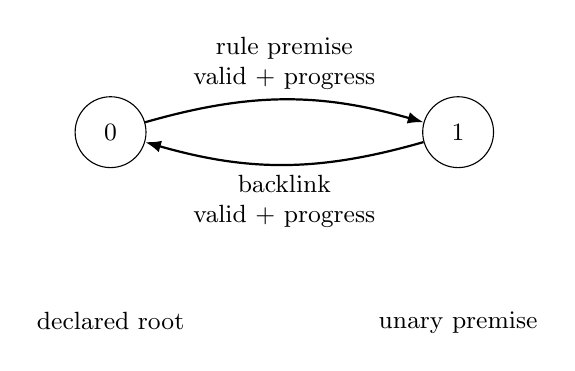
\begin{tikzpicture}[
  n/.style={circle,draw,minimum size=9mm,font=\small},
  arr/.style={-{Latex[length=2mm]},thick},
  lab/.style={font=\small,align=center}
]
\node[n] (n0) {0};
\node[n,right=35mm of n0] (n1) {1};
\draw[arr] (n0) to[bend left=16] node[lab,above]{rule premise\\valid + progress} (n1);
\draw[arr] (n1) to[bend left=16] node[lab,below]{backlink\\valid + progress} (n0);
\node[lab,below=17mm of n0] {declared root};
\node[lab,below=17mm of n1] {unary premise};
\end{tikzpicture}
\caption{The shape of the artificial two-node teaching cycle from
\file{SP/Examples.v}.  The strict progress labels, not the circular shape
alone, make the cycle acceptable.}
\label{fig:teaching-cycle}
\end{figure}

\soundlim

\code{label_at} falls back to the graph root at an invalid index, but this is
not a loophole: every accepted target is separately bounds-checked before the
label comparison matters.  This illustrates a common executable pattern in the
framework: total helper functions are surrounded by acceptance checks carrying
the real invariant.

A backlink may compare labels modulo \file{SP}'s erased tags and constraints,
yet its packaged rule conclusion and premise still undergo exact
\code{judgment_eqb} checks.  Search currently supplies
\code{exact_backlink_rule goal}, whose premise is exactly \code{goal}; in
practice the search backlink is therefore exact despite the more permissive
framework hook.

\section{Relational closure and the global progress check}

\mathintent

For trace relations, use the two-element slope algebra
\(\{\mathsf{Stay},\mathsf{Decrease}\}\), with decrease dominating composition
and union.  If a path carries \(a\mathrel{\mathsf{Stay}}b\) followed by
\(b\mathrel{\mathsf{Decrease}}c\), the composed arc is decreasing.  A closed
graph path is globally progressing when its composed relation has some
decreasing diagonal \(t\mathrel{\mathsf{Decrease}}t\).  Saturating finite graph
paths and tag relations makes this condition executable.

This is a finite-graph presentation of the global trace condition: an infinite
path through a finite graph revisits a node; the corresponding loop must carry
strict progress on a trace.  It is the regular-proof version of infinite
descent discussed by Brotherston and Simpson
\cite{brotherston2011sequent}.

\rocqreal

\file{Cyclic/Relations.v} implements the algebra.  The function
\path{slope_join} makes \code{Decrease} dominant, and \path{put_arc} merges
duplicate source/target keys.  The function \path{relation_compose} composes
compatible arcs.  The function \path{relation_closure} iterates composition
until equality or supplied fuel is exhausted.  The analogous
\path{path_closure} composes relations whose graph endpoints meet.  Finally:
\[
\src{Cyclic/Relations.v}{relational_trace_check}
=\mathsf{forallb}(\mathsf{loop\_relation\_ok},
                  \mathsf{path\_closure}(\cdots)).
\]
A loop is accepted when the closure of its tag relation contains a decreasing
diagonal.  Non-loop paths impose no check at this final stage.

The framework converts each graph edge into a \code{path_relation}; valid pairs
become arcs and membership in \code{edge_progress} selects their slope.
\src{Cyclic/Framework.v}{relation_fuel} is
\(1+3^{w^2}\) for \(w\) distinct graph tags, and
\code{graph_path_fuel} is \(1+n^2\) times the relation fuel for \(n\) nodes.
These finite bounds are then passed to \code{relational_trace_check} by
\code{relational_check}.

The regression examples in \file{Cyclic/Relations.v} make the intended algebra
concrete: composing stay with decrease produces a decreasing diagonal; a
decreasing one-node loop passes; a flat one-node loop fails.

\soundlim

The relational closure check is part of acceptance, but the generic
\src{Cyclic/Framework.v}{certificate_sound} proof does not consume a theorem
reflecting this Boolean closure.  Instead, it consumes the explicit finite
trace witness described next.  Therefore one should describe
\code{relational_check} as an additional conservative acceptance condition,
not as the logical premise used by the final infinite-descent proof.

The fuel formulas are deliberately generous finite-state saturation bounds and
can be expensive.  Their presence does not make graph search complete; graph
construction and witness enumeration are independently bounded and incomplete.

\section{Finite trace witnesses}

\mathintent

A finite witness chooses, at each node \(i\), either no trace tag yet or one
tag \(t_i\), plus an auxiliary potential \(p_i\in\Nat\).  On an edge
\(i\to j\) that leads into a live region, the transition conditions are:

\begin{center}
\begin{tabular}{lll}
\toprule
source choice & target choice & obligation\\
\midrule
none & none & \(p_j<p_i\)\\
none & some tag & true (start following a trace)\\
some tag & none & false (a selected trace may not disappear)\\
\(a\) & \(b\) & \((a,b)\in V_e\) and
  \(((a,b)\in P_e)\lor p_j<p_i\)\\
\bottomrule
\end{tabular}
\end{center}

The auxiliary potential lets the witness traverse finitely many non-progress
edges, or delay trace selection, without pretending those steps decrease the
semantic rank.  A node is \emph{live} if it begins a path of length equal to the
number of stored nodes; in a finite graph this is enough to reach a cycle.

\rocqreal

The record \src{Cyclic/Framework.v}{trace_witness} stores two total functions:
\code{witness_tag : nat -> option nat} and
\code{witness_potential : nat -> nat}.  \code{option_tag_wfb} checks that a
selected tag belongs to a live node's judgment.  \code{trace_transitionb} is
the Boolean form of the four-row table, while \code{trace_transition} is its
propositional form.  \code{witness_check} checks all relevant outgoing edges.

The combined Boolean acceptance function is exactly
\begin{equation}
 \mathsf{raw\_check}(g,tw)=
 \mathsf{structural\_check}(g)\land
 \mathsf{relational\_check}(g)\land
 \mathsf{witness\_check}(g,tw).
 \label{eq:raw-check}
\end{equation}

\soundlim

The witness is global data, not one independent tag choice per path.  One
choice function must satisfy every checked live edge.  This restriction is
convenient for a finite soundness certificate and may reject graphs that admit
a more path-dependent infinitary trace argument.

Edges into non-live regions impose no witness transition.  This is sound for
the intended countermodel argument because a false node is later proved live;
finite dead regions cannot host the infinite sequence used for contradiction.

\section{Certificates and lexicographic infinite descent}

\mathintent

Assume the root is false in some world.  At every false graph node, local
countermodel propagation chooses a false successor and respects its edge
relation.  A finite witness then gives a measure that strictly decreases at
each chosen step.  Such an infinite descent is impossible in a well-founded
order, so the root has no countermodel.

Two phases must be combined.  Before a trace has been selected, use the
auxiliary potential.  After selection, use the pair of semantic tag rank and
auxiliary potential:
\[
 M(i,w)=
 \begin{cases}
   \mathsf{Before}(p_i), & t_i=\mathsf{None},\\
   \mathsf{Following}(\rank(J_i,w,t_i),p_i),&t_i=\mathsf{Some}(t_i).
 \end{cases}
\]
Encode these as \((1,(p_i,0))\) and
\((0,(\rank(J_i,w,t_i),p_i))\), ordered lexicographically.  Starting a trace
strictly decreases the leading phase bit.  A progressing pair decreases the
semantic rank.  A merely valid pair cannot increase that rank and must decrease
the auxiliary potential.  Before selection, the auxiliary potential decreases.

\rocqreal

The \src{Cyclic/Framework.v}{certificate} record contains the graph and
witness, root existence and label evidence, and three semantic obligations:

\begin{itemize}
\item \code{cert_false_live}: every bounded false node is live;
\item \code{cert_advance}: every bounded false node has a bounded false
      successor whose edge relation is respected;
\item \code{cert_trace_transition}: every edge into a live node follows the
      finite witness.
\end{itemize}

These fields are not Booleans.  They are dependent proof terms checked by the
kernel.  \src{Cyclic/Framework.v}{measure_lt_wf} obtains well-foundedness from
nested strict lexicographic products of \(<\) on natural numbers.

\src{Cyclic/Framework.v}{certificate_step_decreases} combines
\code{cert_advance}, target liveness, witness transition, and
\code{respects_edge} to produce a false successor with smaller combined
measure.  The four cases exactly match the preceding transition table.

Finally, \src{Cyclic/Framework.v}{certificate_sound} assumes a false root,
uses classical double-negation elimination, and performs well-founded induction
on the combined measure.  The step lemma always supplies a smaller false state,
contradicting the induction hypothesis.  Hence
\[
  \mathsf{check\_certificate}(c)=\mathsf{true}
  \quad\Longrightarrow\quad
  \Valid(\mathsf{root}(c)).
\]

\soundlim

There is a subtle but crucial implementation fact: the proof of
\code{certificate_sound} introduces the Boolean-check hypothesis with an
anonymous pattern and does not use it.  Soundness resides in the semantic
fields already stored in \code{certificate}.  The check is valuable as an
acceptance interface and is essential to the automated constructor developed
in \file{SP/Certification.v}; it is not an oracle that makes an arbitrary
certificate sound.

This separation is strong proof engineering.  A manually constructed
certificate must provide the hard semantic fields directly.  A computed graph
obtains them only through proved reflection lemmas.  In neither case can a
Boolean value inhabit those dependent fields without a theorem.

\chapter{The implemented separation-logic rules}
\label{ch:rules}

This chapter states each mathematical rule before its Rocq package.  Empty edge
information is used whenever the rule makes no trace claim.

\section{Identity and tag erasure}

\mathintent

Exact identity is the axiom
\[
  \infer[\mathrm{id}]{F\vdash F}{}
\]
for a fixed definition environment.  Tag erasure is the one-way axiom
\[
  \infer[\mathrm{erase}]{F\vdash \lfloor F\rfloor}{}
\]
where \(\lfloor F\rfloor\) removes all ordinal constraints and changes every
predicate tag to anonymous.  This direction is sound because a named tag adds
an upper-bound obligation, while an anonymous tag imposes none.  The reverse
direction is not generally valid.

\rocqreal

\src{SP/Rules.v}{identity_valid} proves implication by assumption, and
\code{identity_axiom} packages it.  The tag-erasure proof proceeds from
predicate occurrences outward: \code{erased_predicate_holds} retains the ranked
membership witness and discards its bound; \code{spatial_erase_tags} lifts this
over separating conjunction; \code{heap_erase_tags_holds} lifts it to symbolic
heaps; and \code{tag_erasure_valid} selects the erased image of the original
disjunct.  \code{tag_erasure_axiom} packages the theorem.

\soundlim

Exact identity uses structural formula equality, not semantic normalization.
The erasure axiom requires the succedent to be exactly the computed erasure of
the antecedent.  It is not a general ``ignore tags whenever convenient'' rule,
and it never adds a missing constraint or tag bound.

\section{Ex falso from an explicit contradiction}

\mathintent

For any right formula \(R\), an inconsistent left formula proves the sequent:
\[
  \infer[\bot L]{L\vdash R}{\mathsf{inconsistent}(L)}.
\]
The implemented decision procedure recognizes only a direct reflexive
disequality \(t\neq t\) in every disjunct of \(L\).  This suffices because the
pure conjunction of the selected disjunct would contain a false atom.

\rocqreal

\src{SP/Syntax.v}{heap_inconsistentb} searches for an atom on which
\code{pure_reflexive_contradiction} succeeds.  Formula inconsistency is
\code{forallb} over disjuncts, including the vacuous truth for an empty
disjunction.  \src{SP/Rules.v}{heap_inconsistentb_sound} reflects the recognized
atom into semantic contradiction; \code{formula_inconsistentb_sound} lifts the
argument through the selected disjunct; \code{ex_falso_valid} and
\code{ex_falso_axiom} close the sequent.

\soundlim

The test does not discover contradictions such as \(x=y\land x\neq y\), alias
conflicts between two points-to atoms, impossible null allocation, or
inconsistent tag constraints.  Those may be semantically false, but this axiom
generator returns \code{None} unless the narrow check succeeds.  Again, this is
incompleteness rather than unsoundness.

\section{Right introduction of an inductive predicate}

\mathintent

For a clause \(c=(B\Rightarrow P(\bar x))\) and a substitution \(\sigma\), the
implemented introduction principle is
\[
  \infer[P\mathrm{R}_c]
    {\sigma B\vdash P(\sigma\bar x)}
    {c\in D(P)}.
  \label{rule:pred-intro}
\]
It has no proof-graph premises because the entire instantiated body appears in
the antecedent.  Semantically, any finite set of predicate occurrences in
\(\sigma B\) has a common maximum rank \(n\); the chosen clause then establishes
the head predicate at rank \(n+1\).

\rocqreal

\src{SP/Rules.v}{spatial_formula_has_bound} inducts through the spatial atoms
and combines child ranks with \code{Nat.max}.  The heap-level version is
\path{heap_formula_has_bound}.  In \path{predicate_intro_valid}, satisfaction
of the singleton antecedent produces such a bound.  The proof constructs an
instance of \path{predicate_holds_rank} at \code{S bound}.  It uses the supplied
clause, substitution, and merged valuation, then packages the whole world heap
as the single predicate's owned heap with an empty frame.

\code{predicate_intro_axiom} stores the resulting theorem.  It is called an
axiom instance because it closes a proof-graph leaf, not because the logical
fact is assumed: the field contains the completed Rocq proof.

\soundlim

The rule accepts an untagged singleton predicate on the right and an exactly
matching singleton symbolic heap on the left.  It is not a general right
unfolding inside an arbitrary spatial context.  Search also lacks a companion
left-unfolding rule at this revision.

The common-rank construction ignores named tag bounds in the antecedent after
extracting membership: the resulting right predicate is anonymous, so no new
upper-bound obligation is required.  A tagged conclusion would need a stronger
rule.

\section{Left disjunction and right choice}

\mathintent

Disjunction in the antecedent is eliminated by proving both cases:
\[
 \infer[\lor L]
   {(H\lor T)\vdash R}
   {H\vdash R & T\vdash R}.
 \label{rule:left-disj}
\]
Here \(T\) denotes the disjunction of the remaining symbolic heaps.  A right
disjunction is introduced by choosing a single branch:
\[
 \infer[\lor R_1]
   {L\vdash (H\lor T)}
   {L\vdash H}.
 \label{rule:right-disj}
\]
The second rule is sound but asymmetric; another branch might be provable even
when the first is not.

\rocqreal

\src{SP/Rules.v}{left_disjunction_rule} has two premises built by
\code{left_head_judgment} and \code{left_tail_judgment}.  Its forward theorem
case-analyzes the selected antecedent disjunct.  Its countermodel theorem uses
classical informative excluded middle to decide whether the head-only formula
holds in the countermodel world; it selects the corresponding false premise.

\src{SP/Rules.v}{right_disjunction_rule} has one premise, the head-only
succedent.  Its forward proof embeds a witness for the head into the larger
disjunction.  Its countermodel proof observes that if the larger succedent is
false, the chosen head succedent is false as well.  Both rules use empty trace
edges.

\soundlim

The left rule preserves the original formula constraints on both branches.
Existential witnesses remain local to satisfaction of each premise formula; no
computational witness is transferred between branches.

The right generator only chooses the head disjunct.  It neither produces one
candidate per right disjunct nor backtracks over alternative choices.  This is
one of the most visible sources of search incompleteness.

\section{Exact backlinks and the teaching-only progressing loop}

\mathintent

An exact backlink is semantically an identity step:
\[
  \infer[\mathrm{backlink}]{J}{J}.
\]
For each visible tag \(t\), the edge admits \((t,t)\) as non-increasing and
claims no progress.  Such an edge can participate in a valid cyclic proof only
if progress is supplied elsewhere on every relevant loop.

\rocqreal

\src{SP/Rules.v}{identity_edge} maps visible judgment tags to identity pairs.
\code{identity_edge_respected} proves equality of source and target ranks, and
\code{exact_backlink_rule} packages the unary identity theorem plus its
countermodel step.

The same file also defines \code{progressing_valid_rule}.  Given an independent
proof \(\Valid(J)\), it constructs a unary \(J/J\) rule whose edge declares
\((t,t)\) progressing.  Its countermodel field is discharged ex falso because
a valid conclusion has no countermodel.  \file{SP/Examples.v} uses this rule to
exercise the cyclic checker.

\soundlim

\code{progressing_valid_rule} is not a search rule for discovering inductive
progress.  Its premise is already accompanied by a proof that the conclusion
is valid.  Therefore the two-node example built from it demonstrates graph and
trace plumbing, not a circular proof of a previously unknown separation-logic
entailment.

An exact backlink edge makes no strict progress.  Since the current search
generates no progressing object-logic rules, backlinks cannot by themselves
produce an accepted genuine cyclic search result.  They remain useful
infrastructure for future rules.

\chapter{Executable rule generation}
\label{ch:generation}

\section{One-way ordered matching}

\mathintent

To instantiate Rule~\ref{rule:pred-intro}, search must find a clause whose head
and body match the goal.  The intended computation is matching, not symmetric
unification: variables in the clause pattern may be assigned target terms, but
target variables are treated as syntax.  Lists match position by position and
must have equal length.  The process is deterministic for one clause:
\[
 \mathsf{head}(c)\mathrel{\triangleright}\mathsf{targetArgs}
 \quad\text{then}\quad
 \mathsf{body}(c)\mathrel{\triangleright}\mathsf{targetBody}.
\]
The substitution accumulated by the head match constrains the body match.
Pure atoms must have the same constructor, points-to atoms retain their list
position, and predicates retain both name and list position.

\rocqreal

\file{SP/RuleGeneration.v} implements separate matchers for two terms, pure
atoms, pure lists, points-to atoms, points-to lists, predicates, predicate lists,
and entire heaps.  The heap order is pure atoms, points-to atoms, then predicate
atoms.  The essential shape is:

\begin{lstlisting}[caption={Ordered heap matching; no permutation search occurs.}]
Definition unify_heap pattern target s : option substitution :=
  match unify_pures pattern.(heap_pure) target.(heap_pure) s with
  | Some s1 =>
      match unify_points_list pattern.(heap_points)
                              target.(heap_points) s1 with
      | Some s2 =>
          unify_predicate_list pattern.(heap_predicates)
                               target.(heap_predicates) s2
      | None => None
      end
  | None => None
  end.
\end{lstlisting}

\src{SP/RuleGeneration.v}{predicate_intro_for_clause} first obtains the
membership proof that the clause occurs in the named definition.  It matches
the head, then the body, constructs \code{predicate_intro_axiom}, and finally
checks that this theorem package's complete conclusion is exactly the original
goal.  The final check is a defense against a matcher that produced a
substitution insufficient to reconstruct the intended judgment.

\src{SP/RuleGeneration.v}{first_predicate_intro} tries clauses in definition
order and returns the first candidate.  \code{predicate_intro_candidate} is
defined only for singleton left and right disjunctions, where the right heap is
exactly one predicate and has no pure or points-to atoms.

\soundlim

The matcher does not search permutations of conjunction lists, perform
associative-commutative matching, or solve pure equalities.  This is stricter
than the heap semantics, where cell-list order is erased by permutation in
\code{heap_join}.  A mathematically identical reordering may therefore prevent
generation.

Pattern \code{Var x} can bind either a free or existential variable.  The
utility \src{SP/Automation.v}{existential_substitutionb} recognizes
substitutions that bind only existential variables, but the predicate
introduction generator does not use that filter.  Soundness does not depend on
the filter: \code{predicate_intro_valid} is quantified over every executable
substitution, and the final conclusion equality must hold.  The utility records
a useful side condition for future transformations.

\section{Candidate priority and conservative stubs}

\mathintent

Rule generation should prefer leaf closure over branching.  If more than one
sound axiom applies, any is acceptable; order only affects search behavior.
Ordinary rule candidates may form a list, whose order becomes depth-first
search order.

\rocqreal

\src{SP/RuleGeneration.v}{generate_axiom} uses left-biased \code{first_some} in
this exact priority:
\begin{enumerate}
\item exact identity;
\item explicit pure inconsistency;
\item tag erasure;
\item predicate introduction.
\end{enumerate}
\src{SP/RuleGeneration.v}{generate_rules} returns the optional left-disjunction
candidate followed by the optional right-disjunction candidate.  A disjunction
candidate is created only when at least two symbolic heaps are present.

Seven named generator boundaries currently return \code{None} unconditionally:
\begin{itemize}[nosep]
\item \code{generate_equality_substitution};
\item \code{generate_constraint_simplification};
\item \code{generate_bound_introduction};
\item \code{generate_points_to_instantiation};
\item \code{generate_left_unfolding};
\item \code{generate_right_unfolding}; and
\item \code{generate_partial_backlink}.
\end{itemize}

\soundlim

These stubs are a positive part of the trust story.  An unsupported operation
does not manufacture a graph node and hope a later checker will reject it; it
has no candidate.  Consequently the implemented prover is much smaller than a
full cyclic separation-logic calculus.

The priority list is operational, not logical.  For example, if identity
succeeds, a later predicate-introduction interpretation of the same goal is
never attempted.  This cannot harm soundness, but it can affect proof shape and
future performance extensions.

\chapter{Reflection: from a checked graph to semantic evidence}
\label{ch:reflection}

\section{Why reflection is needed}

\mathintent

A Boolean equation such as \(\mathsf{rawCheck}(g,t)=\mathsf{true}\) is easy to
compute but does not by itself provide the dependent functions required by the
generic certificate.  A reflection layer must prove, once and for all, that the
successful finite checks reveal:

\begin{enumerate}
\item a real root and its exact label;
\item a false successor and countermodel from every false bounded node;
\item liveness of every false bounded node;
\item a propositional trace transition on every relevant edge.
\end{enumerate}

The difficult item is countermodel propagation.  The graph checker knows only
node shape.  The rule package stored at the node knows how to turn a
countermodel of its conclusion into a countermodel of one premise.  Reflection
must align that selected premise with the checked target index and label.

\rocqreal

\file{SP/Certification.v} builds this bridge in layers.  The early lemmas
reflect membership and index-based checks:

\begin{itemize}
\item \code{pair_mem_spec} turns a true pair lookup into \code{In};
\item \code{all_nodes_wfb_from_nth} and \code{structural_node_wfb} recover the
      well-formedness equation for a particular node;
\item \code{structural_root_bound} and \code{structural_root_label} recover
      root evidence;
\item \code{targets_wfb_nth} aligns a premise selected by
      \code{rule_counter_step} with its graph target, bounds proof, and label;
\item \code{node_edge_from_rule_nth} recovers the corresponding proposition
      \code{edge_at}.
\end{itemize}

The main lemma \src{SP/Certification.v}{structurally_checked_advance} analyzes
the payload of a false node.  An open node contradicts structural
well-formedness.  An axiom node contradicts its stored validity theorem.  At a
rule node, \code{rule_counter_step} chooses a false premise and semantic world,
while \code{targets_wfb_nth} locates its checked graph target.  At a backlink
node, the unary target checks provide the same alignment directly.

There is a Rocq-specific dependent-elimination point worth noticing.  The proof
destructs the executable \code{node_at g i} lookup rather than first proving
\(\exists n\) in \code{Prop}.  The desired result contains dependent witnesses
in \code{Type}; eliminating an arbitrary existential proof from \code{Prop}
into such data would be disallowed.  Computing the lookup preserves the needed
information in the eliminable sort.

\soundlim

Structural checking alone gives a false successor, but it does not give an
infinite path for arbitrary nodes.  The lemma
\src{SP/Certification.v}{false_has_path_of_length} iterates the advance theorem
for any finite fuel while maintaining falsity.  Instantiating the length with
the graph size proves \code{structurally_checked_false_live}.  This is why the
certificate's liveness field is restricted to false nodes.

The bridge uses the semantic countermodel theorem stored in every rule package.
If a future generator introduces a rule without a correctly proved
\code{rule_counter_step}, it will fail at construction of the rule instance,
not merely in this reflection proof.

\section{Reflecting the finite witness}

\mathintent

The Boolean trace transition must imply its propositional four-case
counterpart.  That counterpart is consumed by the descent lemma
\path{certificate_step_decreases}.  Whole-graph witness success must then
specialize to an arbitrary actual edge into a live target.

\rocqreal

\src{SP/Certification.v}{trace_transitionb_sound} performs the four-way case
analysis on source and target tag choices.  Boolean pair membership is reflected
through \code{pair_mem_spec}; natural less-than is reflected through
\code{Nat.ltb_lt}.  \code{witness_edges_from_nth} selects the checks for a node
index, and \code{witness_check_transition} selects the particular outgoing edge
and rewrites the target liveness test to true.

With these pieces, \src{SP/Certification.v}{certify_raw_check} constructs the
generic certificate:

\begin{lstlisting}[caption={The semantic certificate is constructed from proved projections.}]
Definition certify_raw_check g tw
    (Hcheck : Cyclic.raw_check g tw = true) : Cyclic.certificate.
Proof.
  refine {| Cyclic.cert_graph := g;
            Cyclic.cert_witness := tw;
            Cyclic.cert_root_bound := ...;
            Cyclic.cert_root_label := ...;
            Cyclic.cert_false_live := _;
            Cyclic.cert_advance := _;
            Cyclic.cert_trace_transition := _ |}.
  (* Fields are discharged by structural and witness reflection lemmas. *)
Defined.
\end{lstlisting}

The public theorem \src{SP/Certification.v}{raw_check_sound} constructs this
certificate and applies generic \code{certificate_sound}.

\soundlim

Equation~\eqref{eq:raw-check} contains three conjuncts.  The certificate
constructor explicitly projects \code{structural_check} and
\code{witness_check}; it does not project or reflect \code{relational_check}.
Nevertheless, callers must supply the full \code{raw_check = true} equation, so
the relational condition is an additional acceptance gate.  The precise
relationship is:

\begin{center}
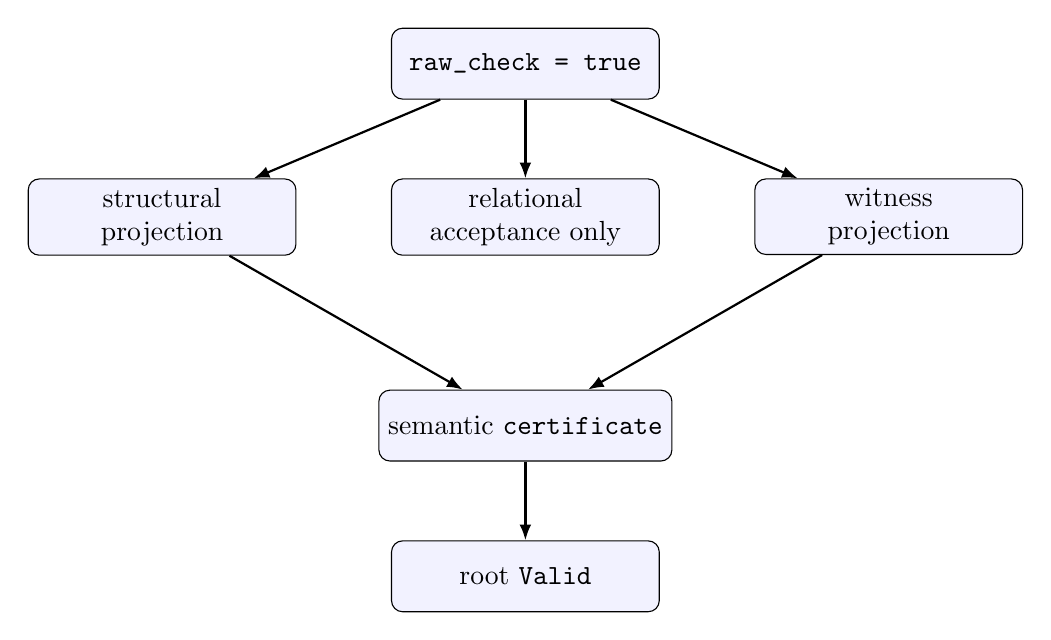
\begin{tikzpicture}[
  b/.style={draw,rounded corners,align=center,minimum height=9mm,
            minimum width=34mm,fill=blue!5},
  arr/.style={-{Latex[length=2mm]},thick}
]
\node[b] (raw) {\code{raw_check = true}};
\node[b,below left=10mm and 12mm of raw] (struct) {structural\\projection};
\node[b,below=10mm of raw] (rel) {relational\\acceptance only};
\node[b,below right=10mm and 12mm of raw] (wit) {witness\\projection};
\node[b,below=17mm of rel] (cert) {semantic \code{certificate}};
\node[b,below=10mm of cert] (valid) {root \code{Valid}};
\draw[arr] (raw) -- (struct);
\draw[arr] (raw) -- (rel);
\draw[arr] (raw) -- (wit);
\draw[arr] (struct) -- (cert);
\draw[arr] (wit) -- (cert);
\draw[arr] (cert) -- (valid);
\end{tikzpicture}
\end{center}

This is stricter than the semantic constructor requires, not weaker.  Removing
the relational check would change which graphs the executable prover accepts,
even though the existing witness-based soundness proof might still apply.
Such a change would therefore be an interface and policy change, not a trivial
proof cleanup.

\section{Acyclic leaves use the same certificate interface}

\mathintent

A one-node graph closed by a valid axiom has no outgoing edge and no infinite
path.  Its structural check passes, and both progress checks are vacuous.  It
should still be usable through the same generic certificate API as a cyclic
graph.

\rocqreal

\src{SP/Certification.v}{axiom_graph} creates the one-node graph.
\code{empty_trace_witness} selects no tag and potential zero everywhere.
\code{axiom_graph_raw_check} proves the full Boolean check by reduction;
\code{certify_axiom} passes that equation to \code{certify_raw_check}.  Search
does not need a special semantic soundness theorem for leaf-only success.

\soundlim

The word ``certificate'' does not imply that the graph is cyclic.  It names the
uniform object consumed by \code{certificate_sound}.  This matters in
Chapter~\ref{ch:vertical}: the benchmark proof is a certified one-node axiom
graph, despite residing in a cyclic-prover architecture.

\chapter{Graph exploration and the public search API}
\label{ch:search}

\section{First-open-node depth-first search}

\mathintent

At each graph state, select a deterministic open node, enumerate successors in
a fixed priority order, and recursively explore each successor before moving to
the next.  A closed graph is a candidate result only after all acceptance checks
and a finite-witness search succeed.  Fuel bounds the number of expansion levels
on one attempt.

\rocqreal

\src{SP/GraphSearch.v}{first_open_from} scans the node list from index zero and
returns the first \code{OpenNode}.  Since rule application appends premises,
this is the first open node in list order, not a heuristic best goal.

For that node, \src{SP/GraphSearch.v}{expand_graph} concatenates successors in
this exact order:
\begin{enumerate}
\item the single candidate from \code{generate_axiom}, if any;
\item exact backlinks to prior indices in ascending order
      \(0,\ldots,i-1\);
\item ordinary generated rules, left-disjunction before right-disjunction.
\end{enumerate}
\src{SP/GraphSearch.v}{bounded_graph_search_from} first tries to check the
current graph.  If it is not accepted and fuel is positive, it recursively
explores each expanded graph with predecessor fuel.  This is a conventional
list-ordered depth-first search.

\begin{figure}[t]
\centering
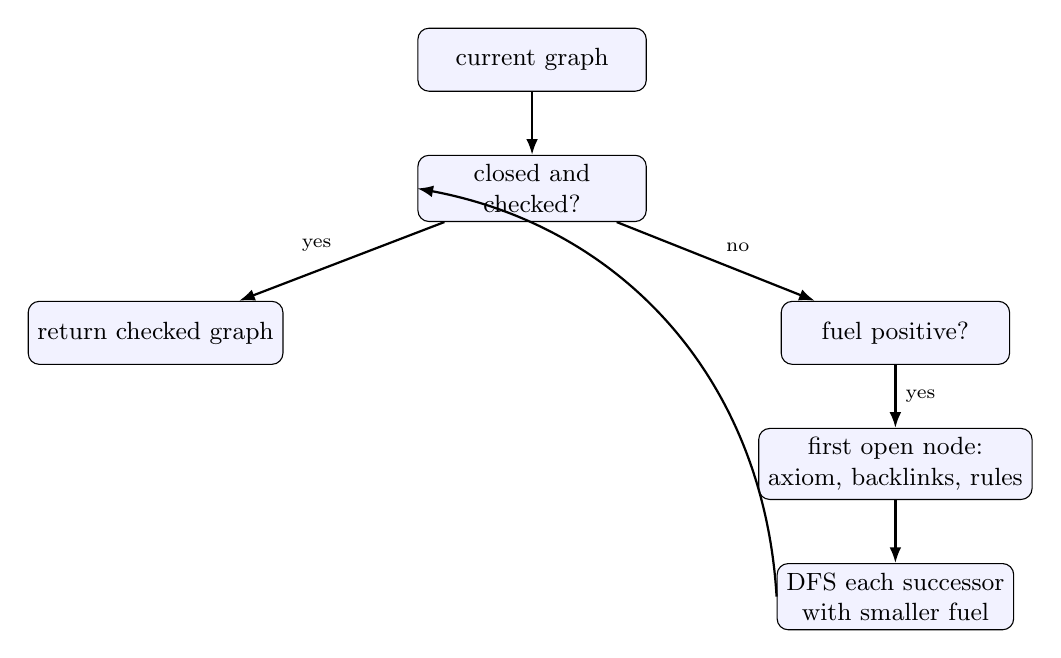
\begin{tikzpicture}[
 b/.style={draw,rounded corners,align=center,minimum width=29mm,
           minimum height=8mm,fill=blue!5,font=\small},
 arr/.style={-{Latex[length=2mm]},thick},node distance=8mm
]
\node[b] (g) {current graph};
\node[b,below=of g] (closed) {closed and\\checked?};
\node[b,below left=10mm and 17mm of closed] (return) {return checked graph};
\node[b,below right=10mm and 17mm of closed] (fuel) {fuel positive?};
\node[b,below=of fuel] (expand) {first open node:\\axiom, backlinks, rules};
\node[b,below=of expand] (dfs) {DFS each successor\\with smaller fuel};
\draw[arr] (g) -- (closed);
\draw[arr] (closed) -- node[above left,font=\scriptsize]{yes} (return);
\draw[arr] (closed) -- node[above right,font=\scriptsize]{no} (fuel);
\draw[arr] (fuel) -- node[right,font=\scriptsize]{yes} (expand);
\draw[arr] (expand) -- (dfs);
\draw[arr] (dfs.west) to[bend right=38] (closed.west);
\end{tikzpicture}
\caption{Operational control flow of \code{bounded_graph_search_from}.}
\label{fig:dfs}
\end{figure}

\soundlim

Fuel is decreased on every graph expansion, not per completed proof branch.
A rule adding two premises consumes one level immediately; closing those
premises may consume further levels.  Search order can therefore determine
whether a proof is found at a fixed depth.

Backlinks are considered before ordinary rules, but a non-progressing closed
cycle fails checking and search continues with later successors.  Because no
generated separation-logic rule currently has a progressing edge, genuine
cyclic success is not expected from this rule set.

\section{Witness enumeration and closed-graph checking}

\mathintent

Given a syntactically closed graph, first try cheap witness guesses.  If those
fail, enumerate every node-local choice from the finite domain consisting of
``no tag'' plus its visible tags, and every potential in a fixed finite range.
Return the first witness that makes the combined checker true.

\rocqreal

\src{SP/GraphSearch.v}{witness_candidates} begins with:
\begin{enumerate}
\item an everywhere-empty tag witness with zero potentials;
\item a heuristic selecting the first visible tag at every live node, again
      with zero potentials;
\item the Cartesian enumeration of tag assignments and potentials.
\end{enumerate}
For a graph of \(n\) nodes, each potential ranges over
\code{List.seq 0 (S n)}, namely \(0,\ldots,n\).  \code{choose_lists} forms
Cartesian products.  The enumeration is complete only for these finite choice
sets, which are sufficient for the intended node-potential witnesses but can be
combinatorially large.

\src{SP/GraphSearch.v}{checked_graph} stores \(g\), \(tw\), and the equation
\(\mathsf{raw\_check}(g,tw)=\mathsf{true}\).  The constructor
\code{check_graph_with_witness} is defined by destructing the Boolean checker,
so the success branch receives the required equation.  \code{check_closed_graph}
also demands that no open node remains.  \code{certify_searched_graph} converts
the result through \code{certify_raw_check}.

\soundlim

The witness enumeration is an acceptance search nested inside proof-graph
search.  Its cost grows as a product of per-node tag choices and \((n+1)^n\)
potential assignments.  The empty and heuristic witnesses are important fast
paths, especially for acyclic graphs where liveness is false and witness
conditions are vacuous.

\section{Iterative deepening and the meaning of \code{solvedb}}

\mathintent

Iterative deepening repeats bounded DFS at depths
\(d_{\min},d_{\min}+1,\ldots,d_{\max}\).  A public result should contain both a
certificate and evidence that its root is the normalized input goal.

\rocqreal

\file{SP/Search.v} defines \code{search_config} with \code{min_depth} and
\code{max_depth}; the default is 1 through 8.  A \code{verified_proof goal}
contains a generic certificate, an equality between its root and
\code{normalize_judgment goal}, and a successful certificate-check equation.
\src{SP/Search.v}{verified_proof_valid} applies generic soundness and rewrites
the root equality.  Since normalization is currently identity, the final
theorem is exactly about \code{goal}.

\code{generated_graph_strategy} runs bounded graph search, reflects the raw
check into a certificate, and uses decidable judgment equality to validate the
root.  \code{search_depths} tries increasing depths; \code{search} computes the
number of attempts from the inclusive interval.  Finally:
\begin{lstlisting}[caption={The Boolean public query and its one-way theorem.}]
Definition solvedb config goal : bool :=
  match search goal config with Some _ => true | None => false end.

Theorem search_sound config goal :
  solvedb config goal = true -> Cyclic.Valid goal.
\end{lstlisting}

\soundlim

There is no converse theorem.  The correct readings are:
\[
\begin{array}{rcl}
\mathsf{solvedb}(c,J)=\mathsf{true}
 &\Rightarrow& J\text{ is semantically valid},\\
\mathsf{solvedb}(c,J)=\mathsf{false}
 &\Rightarrow& \text{no accepted proof was found within this bounded strategy}.
\end{array}
\]
False does not imply invalidity, satisfiability of the antecedent, existence of
a countermodel, or failure at larger depth.  This limitation applies even when
the configured interval has been completely searched.

\chapter{Complete vertical slice:
  \texorpdfstring{\texttt{benchmark\_base\_19\_1}}{benchmark base 19 1}}
\label{ch:vertical}

This chapter follows one judgment through every layer.  It is the most compact
way to see how a mathematical entailment becomes
\src{SP/Search.v}{benchmark_base_19_search_valid}.

\section{The mathematical entailment}

\mathintent

The benchmark is
\begin{equation}
 x\neq z\ \land\ x\pto y\slstar\mathsf{ls}(y,z)
 \quad\vdash\quad
 \mathsf{ls}(x,z).
 \label{eq:base19}
\end{equation}
Compare its antecedent with the recursive clause of Equation~\eqref{eq:ls}:
\[
 u\neq v\ \land\ u\pto e\slstar\mathsf{ls}(e,v)
 \quad\Rightarrow\quad \mathsf{ls}(u,v).
\]
The substitution \(u\mapsto x\), \(v\mapsto z\), \(e\mapsto y\) makes the
clause body exactly the antecedent and the clause head exactly the succedent.
Therefore Rule~\ref{rule:pred-intro} closes the entailment without premises.

Semantically, suppose the left side holds.  The recursive child
\(\mathsf{ls}(y,z)\) has some finite rank \(r\).  There are finitely many
predicate atoms in the body (here, one), so choose a common bound \(n\ge r\).
The recursive clause witnesses \(\mathsf{ls}(x,z)\) at rank \(n+1\), owning the
entire split heap.  That is exactly the proof of
\code{predicate_intro_valid} specialized to this clause and substitution.

\rocqreal

The judgment in \file{SP/Benchmarks.v} is:

\begin{lstlisting}[caption={Exact source for the worked benchmark.}]
Definition benchmark_base_19_1 : judgment :=
  mk_judgment sl_definitions
    (mk_sequent
      (singleton_formula
        (SH [NEQ (F 0) (F 2)] [PTO (F 0) [F 1]]
          [PR "ls" [F 1; F 2]]))
      (singleton_formula (SH [] [] [PR "ls" [F 0; F 2]]))).
\end{lstlisting}

The path through computation is deterministic:

\begin{enumerate}
\item \code{search_at_depth 1} calls \code{generated_graph_strategy} on the
      identity-normalized goal.
\item \code{bounded_graph_search} starts with one open node at index zero.
\item The open graph is not closed, so \code{expand_graph} asks for an axiom.
\item Identity fails, inconsistency fails, and tag erasure fails.  Predicate
      introduction recognizes the singleton right predicate \code{"ls"}.
\item \code{first_predicate_intro} tests \code{ls_clauses} in order.  The base
      equality clause does not reconstruct the target body.  The recursive
      clause matches.
\item Ordered head matching binds its formal endpoints to \code{F 0} and
      \code{F 2}.  Ordered body matching binds \code{E 0} to \code{F 1}; pure,
      points-to, and predicate lists then agree exactly.
\item \code{predicate_intro_axiom} is built from
      \code{predicate_intro_valid}; the complete conclusion equality check
      succeeds.
\item \code{graph_add_axiom} replaces node zero with \code{AxiomNode}.  No new
      node is added, so the graph has exactly one node.
\item On the recursive call with fuel zero, \code{check_closed_graph} runs
      before the fuel case.  The graph is closed.  The empty trace witness
      passes: structure is correct, there are no edge paths or loops, and the
      sole valid axiom node cannot be a live false node.
\item The returned \code{checked_graph} carries the full raw-check equation.
      \code{certify_raw_check} creates the semantic certificate, and root
      equality produces a \code{verified_proof benchmark_base_19_1}.
\end{enumerate}

The source records the computation and the final theorem:

\begin{lstlisting}[caption={From a computed Boolean to semantic validity.}]
Example general_clause_introduction_search :
  solvedb {| min_depth := 1; max_depth := 1 |}
    benchmark_base_19_1 = true.
Proof. vm_compute. reflexivity. Qed.

Theorem benchmark_base_19_search_valid : Cyclic.Valid benchmark_base_19_1.
Proof.
  apply (search_sound {| min_depth := 1; max_depth := 1 |}).
  vm_compute. reflexivity.
Qed.
\end{lstlisting}

\soundlim

The phrase ``one-node certified proof'' is literal: the graph contains a single
axiom node whose validity theorem is predicate introduction.  It is not a
one-node cyclic loop and it uses no backlink.  The cyclic framework still adds
value by giving the leaf a uniform checked-graph and semantic-certificate path.

The example demonstrates one exact clause instance.  It does not show that
arbitrary list-segment entailments, arbitrary reorderings of the body, or the
other eight selected benchmarks are solved.  In particular,
\src{SP/Search.v}{unsupported_open_goal_is_bounded_non_success} computes false
for \code{benchmark_base_01_1} at depth zero and carefully names the result
``bounded non-success.''

\chapter{Examples, tests, and automation utilities}
\label{ch:support}

\section{Accepted and rejected teaching graphs}

\mathintent

Small graphs should test independent boundaries: an acyclic leaf should pass;
a correctly progressing cycle should pass; an open graph, a reflexive backlink,
and a flat cycle should fail for different reasons.

\rocqreal

\file{SP/Examples.v} first packages \(emp\vdash emp\) with
\path{identity_axiom}.  It turns that leaf into a certificate with
\path{certify_axiom}, then applies \path{certificate_sound}.  This is an
ordinary genuine validity theorem and a minimal certificate regression.

The two-node graph in Figure~\ref{fig:teaching-cycle} uses a tagged identity
judgment.  Its judgment is proved valid independently by \code{identity_valid};
that proof is supplied to \code{progressing_valid_rule}.  The graph applies the
rule at node zero and backlinks node one to zero using another instance of the
same progressing rule.  The witness selects tag zero everywhere.  Both edges
claim strict progress, so \code{teaching_cyclic_raw_check} reduces to true and
the generic certificate proves \code{teaching_cyclic_valid}.

The rejected cases separate concerns:
\begin{itemize}
\item \code{rejected_open_graph} fails structural checking;
\item \code{rejected_malformed_backlink} stores a self-backlink and fails the
      non-reflexivity check;
\item \code{rejected_nonprogressing_cycle} uses exact backlink rules on both
      edges, so the global progress condition fails.
\end{itemize}

\soundlim

The cyclic example is intentionally artificial.  Since validity is an input to
the progressing rule, it cannot serve as evidence that search discovered an
inductive cyclic proof.  The genuine search successes explicitly present in
\file{SP/Search.v} are the general exact-identity example and the clause
introduction proof for \code{benchmark_base_19_1}.

\section{Regression tests for generators}

\mathintent

Executable generators need positive and negative unit tests that pin down their
accepted shapes without claiming completeness.

\rocqreal

\file{SP/Tests.v} checks positive generation for identity, explicit
inconsistency, tag erasure, benchmark-19 predicate introduction, left
disjunction, and right disjunction.  It also checks rejection of unmatched
predicate introduction and of right splitting for a singleton succedent.  Two
semantic/syntax units record identity normalization and exact one-cell
points-to ownership.

Most simple tests close by reflexivity; larger reified computations use
\code{vm_compute}.  These are kernel-checked equations about the actual
generators.  They are not external test-runner assertions.

\soundlim

The tests characterize selected cases only.  Their greatest documentary value
is identifying intended generator domains.  For example, the positive left
split test on \code{benchmark_base_21_1} shows that a rule candidate can be
generated; it does not say the resulting branches are both solved.

\section{Verified automation utilities}

\mathintent

Small verified helpers can establish side conditions before a future rule is
implemented.  A strict self-constraint \(t<t\) is inconsistent; substitutions
used for clause-local instantiation may be restricted to existential-domain
bindings; and fresh identifiers can be chosen above the maximum used id.

\rocqreal

\file{SP/Automation.v} provides:
\begin{itemize}
\item \code{constraints_inconsistentb} and its semantic soundness lemma for a
      directly recognized strict self-constraint;
\item \code{existential_substitutionb}, which checks the kind of every binding
      domain;
\item fresh free/existential variable and free-tag constructors using one plus
      a folded maximum;
\item \code{normalization_candidate} and a semantic equivalence proof, which
      is reflexive because normalization is identity.
\end{itemize}

\soundlim

These utilities are not wired into \code{generate_axiom} or
\code{generate_rules} except indirectly through shared syntax and imports.
In particular, inconsistent ordinal constraints do not currently trigger the
ex-falso generator.  A theorem existing in \file{Automation.v} does not imply
that search calls it.

\chapter{Limitations and precise claims}
\label{ch:limitations}

The current implementation is best understood as a small proof-producing core,
not as a complete port of a mature separation-logic prover.  This positioning
matches the historical contrast between a general cyclic proof architecture
and a logic-specific automated procedure
\cite{brotherston2011automated,brotherston2012generic}.

\mathintent

Soundness and completeness answer different questions.  Soundness asks whether
every reported proof denotes a valid entailment.  Completeness asks whether
every valid entailment is eventually reported.  The code establishes the first
for successful search and makes no general claim about the second.

\rocqreal

Table~\ref{tab:limits} collects the operational restrictions that most often
explain non-success.

\begin{longtable}{>{\raggedright\arraybackslash}p{0.20\textwidth}
                  >{\raggedright\arraybackslash}p{0.34\textwidth}
                  >{\raggedright\arraybackslash}p{0.36\textwidth}}
\caption{Explicit limitations of revision
\code{08f6cd8834a3fc22088a064025abb9ee65c7f545}.}
\label{tab:limits}\\
\toprule
Area & What the implementation does & Consequence\\
\midrule
\endfirsthead
\toprule
Area & What the implementation does & Consequence\\
\midrule
\endhead
Identity normalization & \code{normalize_heap}, \code{normalize_formula},
\code{normalize_sequent}, and \code{normalize_judgment} return their input. &
Semantic equivalents are not canonicalized; equality and matching remain
representation-sensitive.\\
\addlinespace
Ordered matching & Clause head, pure atoms, points-to atoms, predicate atoms,
and arguments match in list order, one way from pattern to target. &
No commutative matching, atom permutation, equality solving, or alternative
substitution search is performed.\\
\addlinespace
Right disjunction & The generator chooses only the first symbolic heap in a
multi-disjunct succedent. & A proof requiring another right branch may fail even
when that branch is directly provable.\\
\addlinespace
Backlinks & Search proposes \code{exact_backlink_rule} to earlier nodes; its
edge carries identity valid pairs and no progress pairs. & The current generated
rules cannot create a genuine progressing search cycle.\\
\addlinespace
Unsupported rules & Equality substitution, constraint simplification, bound
introduction, points-to instantiation, left/right unfolding, and partial
backlink generators return \code{None}. & Their names document intended
boundaries; they contribute no proof power at this revision.\\
\addlinespace
Inconsistency & Ex falso recognizes only a direct \(t\neq t\) in every left
disjunct. & Many unsatisfiable antecedents are not closed.\\
\addlinespace
Predicate introduction & The right side must be one untagged predicate in one
heap; the left side must be one heap exactly matching an instantiated clause
body. & Framed, reordered, tagged, or partially unfolded variants are outside
the generator's domain.\\
\addlinespace
Search bounds & Graph DFS is fuel-bounded and iterative deepening stops at the
configured maximum.  Witnesses are enumerated only after graph closure. &
Runtime and result depend on configuration and successor order.\\
\addlinespace
Boolean result & \code{solvedb = true} has theorem \code{search_sound}; no
converse theorem exists. & \code{false} means bounded non-success, never
semantic invalidity.\\
\addlinespace
Input path & Definitions and benchmarks are handwritten reified values. &
There is no parser, parser-correctness theorem, CLI, or OCaml front-end in this
tutorial or module set.\\
\bottomrule
\end{longtable}

\soundlim

The limitations interact.  A valid goal might first require normalization,
then a non-head right choice, then left unfolding, none of which the current
search performs.  Increasing depth cannot compensate for a missing successor.
Conversely, adding more generators without proved rule packages would violate
the central architecture.  Extension should increase the set of theorem-backed
successors, not weaken the checker.

\chapter{Trust boundary and assumptions}
\label{ch:trust}

\mathintent

A proof-producing prover should separate mathematical assumptions, executable
decisions, and external data.  The strongest useful claim is not ``the program
seems to work,'' but ``under the explicitly printed logical assumptions, the
Rocq kernel accepts a theorem whose statement is semantic validity.''

\rocqreal

At the documented revision, rebuilding \file{SP/Search.v} prints:
\begin{quote}\small\ttfamily
Axioms:\\
Description.constructive\_definite\_description :\\
\quad forall (A : Type) (P : A -> Prop),\\
\qquad (exists! x : A, P x) -> \{x : A | P x\}\\
Classical\_Prop.classic : forall P : Prop, P \/ \char`~ P
\end{quote}
for both \code{search_sound} and
\code{benchmark_base_19_search_valid}.  Rebuilding
\file{SP/Examples.v} prints only \code{Classical_Prop.classic} for
\code{teaching_acyclic_valid} and \code{teaching_cyclic_valid}.

The sources of these assumptions are visible.  Generic
\code{certificate_sound} applies classical double-negation elimination.
\file{SP/Rules.v} uses informative excluded middle while selecting the false
branch of the left-disjunction rule; its standard-library construction brings
in constructive definite description.  These are standard-library axioms, not
project-local admitted theorems.

The trusted and checked components can be summarized as follows:

\begin{longtable}{>{\raggedright\arraybackslash}p{0.26\textwidth}
                  >{\raggedright\arraybackslash}p{0.64\textwidth}}
\toprule
Component & Role in the claim\\
\midrule
Rocq kernel and standard library & Check definitions, proof terms,
well-founded orders, list/permutation facts, and the explicitly reported
classical assumptions.\\
\addlinespace
Reified definitions/benchmarks & Handwritten data.  The kernel checks their
types and reductions, but there is no external-parser correspondence theorem.\\
\addlinespace
Rule generators & Computational filters that can return only pre-proved
\code{axiom_instance} or \code{rule_instance} values.\\
\addlinespace
Graph and witness checks & Executable acceptance conditions.  Their useful
semantic projections are justified in \file{SP/Certification.v}.\\
\addlinespace
Relational trace check & Additional executable acceptance filter; not projected
into the semantic certificate used by the final descent proof.\\
\addlinespace
\code{vm_compute} equations & Kernel-accepted computations establishing the
specific Boolean results shown in examples and the benchmark theorem.\\
\addlinespace
Search strategy & Untrusted for completeness and performance claims, but safe
for validity because any returned object must pass the proof-producing path.\\
\bottomrule
\end{longtable}

\soundlim

There are no project-declared axioms or admitted proof holes in the documented
\file{SP} and required \file{Cyclic} source modules.  This observation does not
remove the printed standard-library assumptions.  It also does not certify the
intended transcription of every external benchmark; it certifies the reified
judgments that actually occur in Rocq.

No soundness statement is made about an extracted program after arbitrary
modification, a textual input not connected to the reified term, or a proposed
graph that has not been converted to a \code{verified_proof}.  The public theorem
begins at the actual \code{solvedb} computation over a Rocq \code{judgment}.

\chapter{A theorem-first extension checklist}
\label{ch:extension}

The safest way to extend this prover is to work backward from the theorem that
the new executable candidate must carry.

\mathintent

Suppose a new transformation maps a conclusion \(J\) to premises
\(J_0,\ldots,J_{m-1}\) and edge relations \(e_0,\ldots,e_{m-1}\).  Before
writing a generator, establish:
\begin{align*}
 &\bigl(\forall k<m.\;\Valid(J_k)\bigr)\Rightarrow\Valid(J),\\
 &w\notholds J\Rightarrow
   \exists k,w'.\;w'\notholds J_k\land
   \mathsf{respectsEdge}(J,J_k,w,w',e_k).
\end{align*}
If the rule claims progress, prove strict rank decrease for exactly those
pairs.  If it changes tags or constraints, first prove the corresponding
semantic monotonicity or witness-transport lemma.

\rocqreal

Use the following checklist in order.

\begin{enumerate}[leftmargin=*,label=\textbf{\arabic*.}]
\item \textbf{State the mathematical rule.}  Specify its conclusion, every
premise, and all side conditions without mentioning the search heuristic.

\item \textbf{Prove semantic helper lemmas in \file{SP/Semantics.v} or
\file{SP/Rules.v}.}  Typical obligations concern heap splitting, ranked
unfolding, substitution, tag bounds, or constraint transport.

\item \textbf{Prove the forward theorem.}  Match the type
\code{premises_valid premises -> Valid conclusion}.  Keep this theorem useful
independently of graph search.

\item \textbf{Prove countermodel propagation.}  Construct the dependent premise
index and target world required by \code{rule_counter_step}.  Do not derive it
from an unproved Boolean heuristic.

\item \textbf{Justify edge information.}  Prove \code{respects_edge} for every
selected countermodel step.  Declare a progressing pair only when the semantic
rank is strictly smaller.

\item \textbf{Package a \code{rule_instance} or \code{axiom_instance}.}  At this
point all logical trust is in kernel-checked fields; the generator will only
decide applicability.

\item \textbf{Implement a conservative generator.}  Return \code{None} whenever
a side condition is undecided or false.  Reflect each successful Boolean side
condition with a theorem before constructing the package.

\item \textbf{Check the complete generated conclusion.}  As predicate
introduction does, compare the package conclusion with the requested goal after
matching or normalization.

\item \textbf{Insert the candidate deliberately into priority order.}  Record
whether it branches and how it interacts with axiom, backlink, and existing
rule priority.

\item \textbf{Add focused positive and negative tests.}  Test the generator's
boundary, graph installation, raw checking, and at least one semantic theorem
through \code{search_sound}.

\item \textbf{Inspect assumptions.}  Run \code{Print Assumptions} on the new
public theorem and explain any change from Chapter~\ref{ch:trust}.

\item \textbf{Keep failure modest.}  Unless a decision procedure and
completeness theorem have actually been proved, retain the interpretation of
false as bounded non-success.
\end{enumerate}

\soundlim

A new Boolean check alone does not add proof power.  A new theorem package that
no generator reaches does not add search power.  A new rule that reaches a
graph but cannot produce a global trace witness does not add accepted cyclic
proofs.  The checklist intentionally covers all three boundaries.

For a genuine cyclic separation-logic extension, the pivotal task is a rule
whose \code{rule_counter_step} exposes a strictly decreasing ranked predicate
trace.  Once that local fact is packaged as edge progress, the existing graph,
relational, witness, reflection, and lexicographic-descent machinery can be
reused.

\appendix

\chapter{Mathematics-to-Rocq correspondence}
\label{app:correspondence}

\begin{longtable}{>{\raggedright\arraybackslash}p{0.28\textwidth}
                  >{\raggedright\arraybackslash}p{0.31\textwidth}
                  >{\raggedright\arraybackslash}p{0.31\textwidth}}
\caption{Quick correspondence between the mathematical presentation and source
symbols.}\\
\toprule
Mathematical object & Rocq realization & Important detail\\
\midrule
\endfirsthead
\toprule
Mathematical object & Rocq realization & Important detail\\
\midrule
\endhead
Location and null & \src{SP/Semantics.v}{location},
\code{nil_location} & Both are naturals; null is zero.\\
Finite partial heap & \code{concrete_heap}, \code{heap_wf} & Association list
with no duplicate address in a world.\\
Disjoint union \(h_1\uplusd h_2=h\) & \code{heap_disjoint}, \code{heap_join} &
Join uses permutation of list concatenation.\\
Exact \(x\pto\bar y\) & \code{points_to_holds} & Non-null address and exactly
one cell.\\
\(emp\) and separating conjunction & \code{spatial_holds_with} & Empty atom
list owns \code{[]}; recursion splits owned heap and frame.\\
Pure conjunction & \code{pures_hold} & Recursive conjunction over a list.\\
Symbolic heap & \code{symheap}, \code{symheap_holds_with} & Pure part plus
spatial fold of points-to atoms followed by predicates.\\
Disjunction & \code{formula_heaps}, membership in \code{formula_holds} & Empty
list denotes false; a selected heap is existential.\\
Existential witnesses & \code{merge_valuation}, \code{merge_tag_valuation} &
Selected once per formula satisfaction derivation.\\
Finite predicate approximant & \code{predicate_holds_rank} & Rank zero is
false; children of rank \(S n\) have some rank at most \(n\).\\
Tag upper bound & \code{tag_bounds_rank} & Anonymous is unconstrained; named
rank is bounded by its valuation.\\
Ordinal constraint & \code{constraint_holds} & Natural-number \(<\) or
\(\le\), not transfinite arithmetic.\\
Entailment validity & \code{sequent_holds}, \code{denote},
\code{Cyclic.Valid} & Universal quantification over well-formed worlds.\\
Non-increasing/progress pair & \code{edge_valid}, \code{edge_progress},
\code{respects_edge} & Progress pairs must also be valid pairs.\\
Local inference rule & \code{rule_instance} & Contains both forward validity
and countermodel propagation.\\
Regular derivation & \code{graph}, \code{node_kind} & Finite index-addressed
graph with explicit backlinks.\\
Global trace condition & \code{relational_check}, \code{witness_check} & Both
are required by \code{raw_check}.\\
Trace start/continuation & \code{trace_witness}, \code{trace_transition} &
Optional selected tag plus auxiliary natural potential.\\
Infinite descent measure & \code{descent_measure}, \code{measure_lt} & Phase,
semantic rank, and potential are lexicographically ordered.\\
Proof certificate & \code{Cyclic.certificate} & Stores executable data and
dependent semantic evidence.\\
Reflection & \code{certify_raw_check} & Projects structure and witness success
into certificate fields.\\
Bounded theorem search & \code{bounded_graph_search_from}, \code{search_depths}
& First-open-node DFS followed by iterative deepening.\\
Successful Boolean query & \code{solvedb}; theorem \code{search_sound} & Only
the true direction has a validity theorem.\\
\bottomrule
\end{longtable}

\chapter{Module and symbol index}
\label{app:index}

\begin{longtable}{>{\raggedright\arraybackslash}p{0.25\textwidth}
                  >{\raggedright\arraybackslash}p{0.65\textwidth}}
\caption{All \file{SP} modules and the necessary \file{Cyclic} modules.}\\
\toprule
Module & Symbols and role\\
\midrule
\endfirsthead
\toprule
Module & Symbols and role\\
\midrule
\endhead
\file{Cyclic/Relations.v} & \code{slope}, \code{arc},
\code{relation_compose}, \code{relation_closure}, \code{path_relation},
\code{path_closure}, \code{relational_trace_check}.  Executable two-slope
relation and graph-path closure algebra.\\
\addlinespace
\file{Cyclic/Framework.v} & \code{THEORY}, \code{Make}, \code{Valid},
\code{edge_info}, \code{respects_edge}, \code{rule_instance},
\code{axiom_instance}, \code{graph}, graph builders, \code{structural_check},
\code{relational_check}, \code{trace_witness}, \code{witness_check},
\code{raw_check}, \code{certificate}, \code{certificate_step_decreases},
\code{certificate_sound}.\\
\addlinespace
\file{SP/Syntax.v} & Reified variables, terms, tags, constraints, pure and
spatial atoms, formulas, clauses, definitions, judgments, decidable equality,
tag erasure, substitution, matching primitives, freshening, identity
normalization, inconsistency checks, visible tags, lookup, and constructors.\\
\addlinespace
\file{SP/Semantics.v} & \code{concrete_heap}, \code{heap_wf},
\code{heap_join}, valuations, exact points-to, \code{spatial_holds_with},
\code{predicate_holds_rank}, tag bounds, constraints, \code{formula_holds},
\code{world}, \code{denote}, \code{SeparationLogicTheory}, and the local
\code{Cyclic} functor instance.\\
\addlinespace
\file{SP/Rules.v} & Identity, tag erasure, explicit ex falso, common-rank
lemmas, predicate introduction, left disjunction, right choice, exact backlink,
and the independently-valid progressing teaching rule.\\
\addlinespace
\file{SP/Automation.v} & Strict self-constraint rejection,
existential-substitution check, fresh identifiers, and identity normalization
equivalence.\\
\addlinespace
\file{SP/Certification.v} & Structural reflection, countermodel advance,
false-node liveness, witness reflection, \code{certify_raw_check},
\code{raw_check_sound}, and uniform one-node axiom certificates.\\
\addlinespace
\file{SP/RuleGeneration.v} & Ordered one-way heap matcher; identity,
inconsistency, erasure, and predicate-introduction axiom candidates; left and
right disjunction rule candidates; named unsupported stubs.\\
\addlinespace
\file{SP/GraphSearch.v} & First-open-node selection, successor priority,
backlink enumeration, tag/potential witness enumeration, \code{checked_graph},
bounded DFS, and searched-graph certification.\\
\addlinespace
\file{SP/Definitions.v} & Hand-reified predicate libraries:
\code{sl_definitions}, \code{atva_definitions}, and
\code{songbird_definitions}; 38 entries in the main library.\\
\addlinespace
\file{SP/Benchmarks.v} & Nine selected reified entailments and
\code{selected_benchmarks}, including \code{benchmark_base_19_1}.\\
\addlinespace
\file{SP/Examples.v} & Genuine acyclic identity certificate; artificial
progressing two-node teaching graph; rejected open, self-backlink, and
non-progressing graphs; printed assumptions.\\
\addlinespace
\file{SP/Tests.v} & Positive and negative generator equations plus normalization
and exact points-to regression examples.\\
\addlinespace
\file{SP/Search.v} & \code{search_config}, \code{verified_proof},
\code{verified_proof_valid}, generated graph strategy, iterative deepening,
\code{solvedb}, \code{search_sound}, genuine search computations, and
\code{benchmark_base_19_search_valid}.\\
\bottomrule
\end{longtable}

\chapter{End-to-end audit checklist}
\label{app:audit}

When reading a claimed success in this codebase, the following compact audit
reconstructs the theorem path without replaying every proof.

\begin{enumerate}[leftmargin=*]
\item Identify the exact \code{judgment}: definition environment, antecedent,
succedent, tags, and constraints.
\item Determine which candidate wins \code{generate_axiom}; if none wins, list
the backlinks and \code{generate_rules} candidates in their real order.
\item For every installed rule, inspect both \code{rule_theorem} and
\code{rule_counter_step}; for every axiom, inspect \code{axiom_theorem}.
\item Check whether the graph is acyclic, a genuine progressing cycle, or an
artificial cycle built from an independently valid judgment.
\item Expand \code{raw_check} into structure, relational closure, and witness
checks.  Record the actual witness candidate that succeeds.
\item Follow \code{certify_raw_check}: structure gives root, liveness, and
advance; the witness check gives trace transitions; the relational check is an
additional acceptance condition.
\item Apply \code{certificate_sound} and then the root equality stored in
\code{verified_proof}.  Only here state semantic validity of the input goal.
\item If computation returns \code{None} or \code{solvedb = false}, report the
depth interval and say only ``bounded non-success.''
\item Run \code{Print Assumptions} on the exported theorem and compare with
Chapter~\ref{ch:trust}.
\end{enumerate}

For \code{benchmark_base_19_search_valid}, this audit collapses to a particularly
clean chain:
\[
\begin{aligned}
&\text{recursive \(\mathsf{ls}\) clause matches the antecedent}\cr
&\Longrightarrow \text{theorem-backed predicate-introduction axiom}\cr
&\Longrightarrow \text{one-node closed graph}\cr
&\Longrightarrow \text{empty witness and vacuous loop checks}\cr
&\Longrightarrow \text{reflected semantic certificate}\cr
&\Longrightarrow \Valid(\texttt{benchmark\_base\_19\_1}).
\end{aligned}
\]

\backmatter
\chapter*{Conclusion}
\addcontentsline{toc}{chapter}{Conclusion}

The \file{SP} development is a compact demonstration of proof-producing
automation.  Its heap semantics is exact and ranked; its rule packages contain
both forward validity and countermodel propagation; its finite graphs are
checked for structure and two forms of global progress; and its reflection
layer converts a successful computation into the semantic evidence required by
a generic lexicographic infinite-descent theorem.

The most important negative fact is equally clear: the current search calculus
is intentionally incomplete.  Identity normalization, ordered matching, one
right choice, exact non-progressing backlinks, and explicit \code{None} stubs
leave many valid entailments outside its reach.  That boundary is safe because
the public API proves only the success direction.  The result is a useful base
for theorem-first extension: add semantic lemmas, package a locally sound rule
with a countermodel step, expose it through a conservative generator, and let
the existing graph-to-certificate path do the rest.

\begin{thebibliography}{9}

\bibitem{reynolds2002separation}
John C. Reynolds.
\newblock Separation logic: A logic for shared mutable data structures.
\newblock In \emph{Proceedings of the 17th Annual IEEE Symposium on Logic in
Computer Science (LICS 2002)}, pages 55--74. IEEE Computer Society, 2002.
\newblock \href{https://doi.org/10.1109/LICS.2002.1029817}%
{doi:10.1109/LICS.2002.1029817}.

\bibitem{brotherston2011automated}
James Brotherston, Dino Distefano, and Rasmus Lerchedahl Petersen.
\newblock Automated cyclic entailment proofs in separation logic.
\newblock In Nikolaj Bj{\o}rner and Viorica Sofronie-Stokkermans, editors,
\emph{Automated Deduction -- CADE-23}, volume 6803 of \emph{Lecture Notes in
Computer Science}, pages 131--146. Springer, 2011.
\newblock \href{https://doi.org/10.1007/978-3-642-22438-6_12}%
{doi:10.1007/978-3-642-22438-6\_12}.

\bibitem{brotherston2011sequent}
James Brotherston and Alex Simpson.
\newblock Sequent calculi for induction and infinite descent.
\newblock \emph{Journal of Logic and Computation}, 21(6):1177--1216, 2011.
\newblock \href{https://doi.org/10.1093/logcom/exq052}%
{doi:10.1093/logcom/exq052}.

\bibitem{brotherston2012generic}
James Brotherston, Nikos Gorogiannis, and Rasmus Lerchedahl Petersen.
\newblock A generic cyclic theorem prover.
\newblock In Ranjit Jhala and Atsushi Igarashi, editors,
\emph{Programming Languages and Systems: 10th Asian Symposium, APLAS 2012},
volume 7705 of \emph{Lecture Notes in Computer Science}, pages 350--367.
Springer, 2012.
\newblock \href{https://doi.org/10.1007/978-3-642-35182-2_25}%
{doi:10.1007/978-3-642-35182-2\_25}.

\end{thebibliography}

\end{document}
